\documentclass[a4paper,12pt]{article}
\usepackage{graphicx}
\usepackage{amsmath, amssymb}
\usepackage{float}
\usepackage{subcaption}
\usepackage{siunitx}
\usepackage{hyperref}
\usepackage{siunitx}
\title{\textbf{Bode Plot Analysis of RC Circuits}}
\author{EE24BTECH11054- Sai Akshitha Suguru\\EE24BTECH11055- Sai Akhila Reddy Turpu}
\date{\today}

\begin{document}

\maketitle

\section{Objective}
\begin{itemize}
    \item Analyze the frequency response of different RC circuits:
    \begin{itemize}
        \item Single RC circuit
        \item Cascaded RC circuit
        \item Twice-cascaded RC circuit
    \end{itemize}
    \item Derive the transfer function $H(s)$ for each case.
    \item Apply logarithmic transformation and simplify the expressions.
    \item Generate magnitude and phase Bode plots to understand system behavior.
\end{itemize}

\section{Theory}

\subsection{Transfer Function $H(s)$}
The transfer function $H(s)$ is determined for each RC circuit using circuit analysis techniques. Then, the logarithmic transformation is applied to simplify the expressions for magnitude and phase calculations.

\subsection{Bode Plot Analysis}
Bode plots represent the logarithmic magnitude $\log |H(s)|$ vs. $\log \omega$ and the phase response. These plots are useful for understanding the frequency-dependent behavior of the circuits.

\section{Experimental Setup}

\subsection{Materials Required}
\begin{itemize}
    \item Resistors and capacitors for each circuit configuration.($R=100\si{\ohm}$ and $C=100\si{\micro\farad}$)
    \item A signal generator to provide input voltage.
    \item An oscilloscope to measure the output voltage.

\end{itemize}

\subsection{Procedure}
\begin{itemize}
    \item Assemble the circuit configurations as per the given schematics.
    \item Apply an input signal and measure the output at different frequencies.
    \item Record the voltage gain and phase shift at each frequency.
    \item Compute the transfer function $H(s)$ for each configuration.
    \item Apply logarithmic transformation to obtain magnitude and phase equations.
    \item Plot the magnitude and phase Bode plots.
\end{itemize}

\section{Results and Discussion}

\subsection{Case 1: Single RC Circuit}
\subsubsection{Circuit Diagram}
\begin{figure}[H]
    \centering
    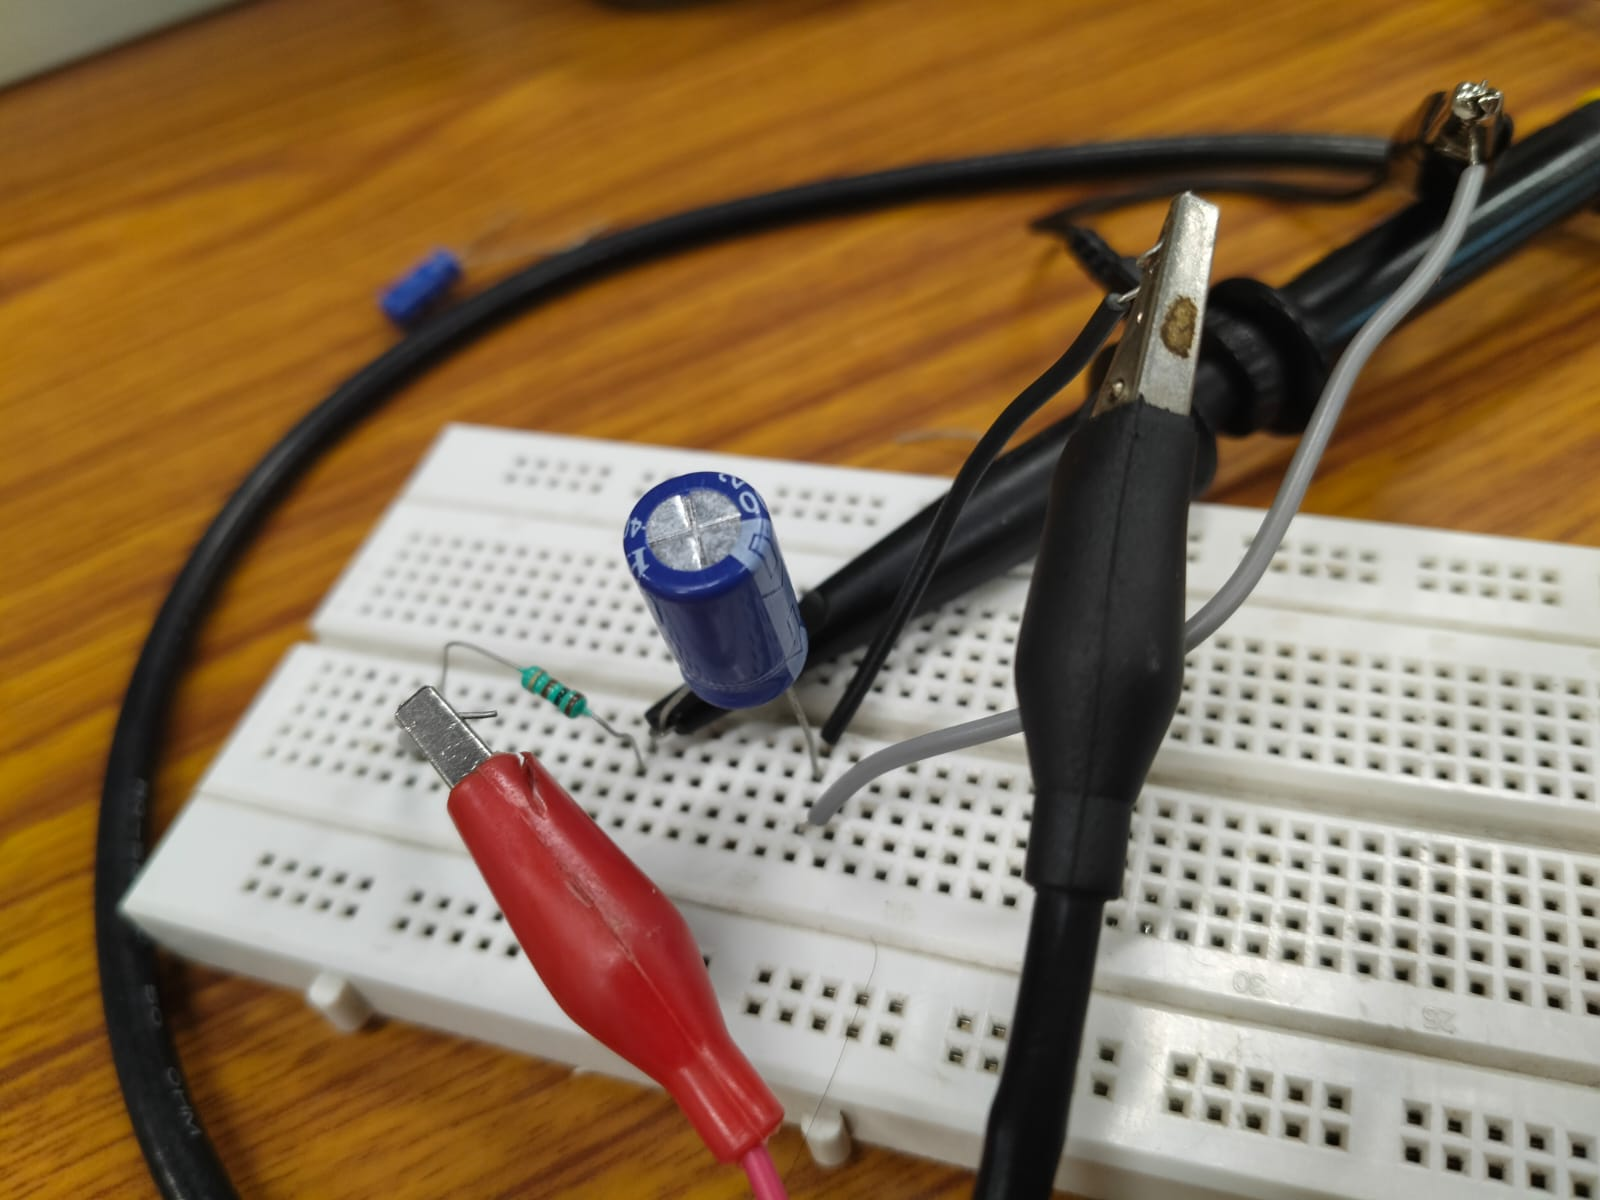
\includegraphics[width=0.7\textwidth]{fig/rc1.jpeg} % Replace with actual file
    \caption{RC Circuit Diagram}
\end{figure}

\subsubsection{Transfer Function}
Derived as:
\begin{equation}
    H(s) = \frac{1}{1 + sRC}
    H(j\omega)=\frac{1}{1+\omega RCj}
\end{equation}
Applying logarithm:
\begin{align}
    \log |H(j\omega)| &= -\frac{1}{2}\log(1 + R^2C^2\omega^2)\\
    \log |H(j\omega)| &= -\log(RC)-\frac{1}{2}log(\frac{1}{R^2C^2}+\omega^2)\\
    20\log |H(j\omega)| &= -20log(RC) -10\log(\frac{1}{R^2C^2}+\omega^2)
\end{align}
For nth order circuit, we get 
\begin{equation}
    \phi = -n\tan^{-1}(RC\omega)
\end{equation}
We get phase to be :
\begin{equation}
    \phi =-\tan^{-1}(RC\omega)
\end{equation}
\subsection{Oscilloscope- Practically measured VPP}
\subsubsection{w = 10}
\begin{figure}[H]
    \centering
    \begin{minipage}{0.48\textwidth}
        \centering
        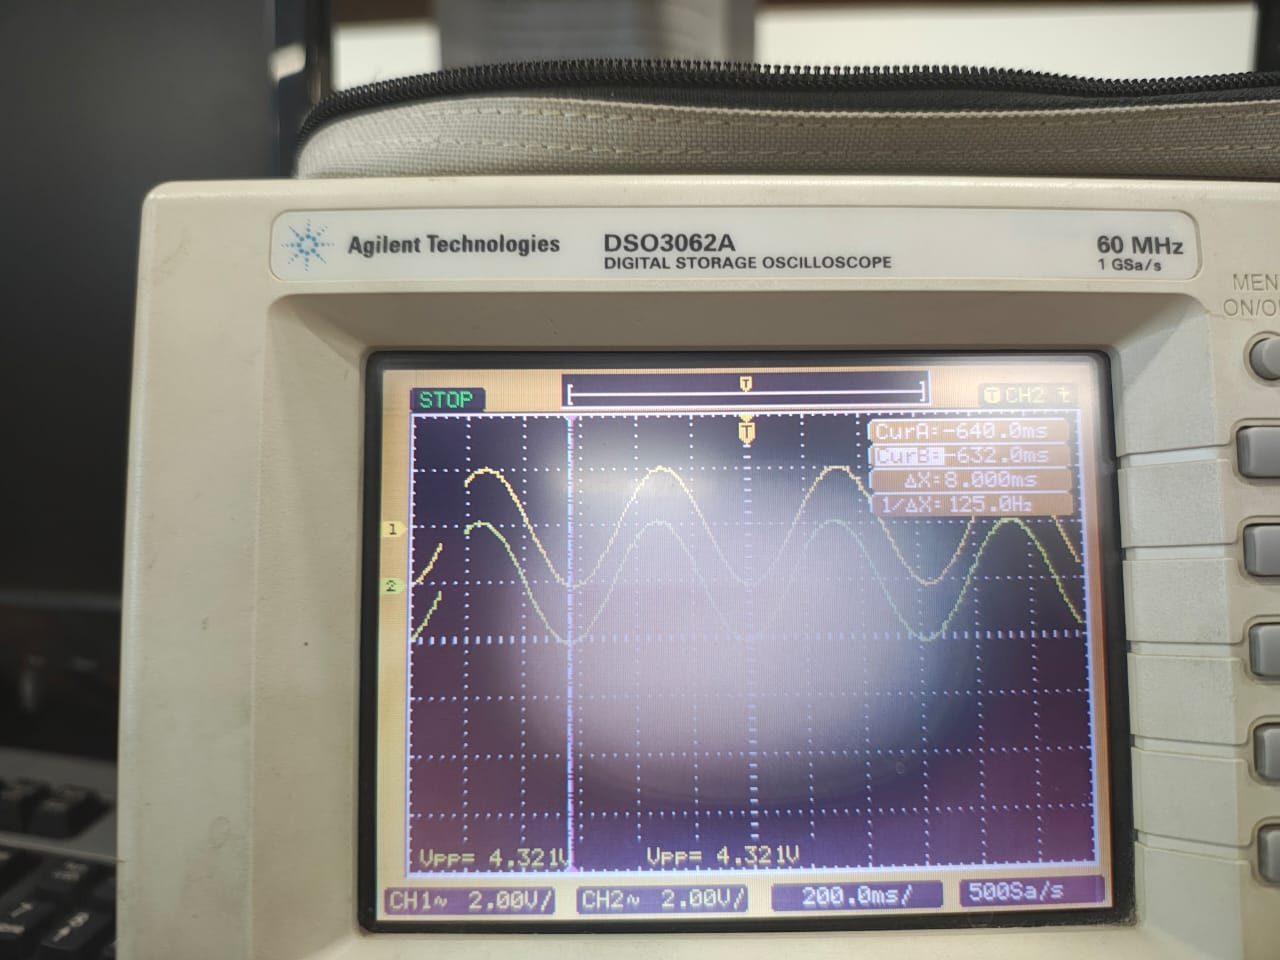
\includegraphics[width=\textwidth]{fig/1w10o.jpeg} % Replace with actual file
        \caption{Oscilloscope Reading for w = 10}
    \end{minipage}
    \hfill
    \begin{minipage}{0.48\textwidth}
        \centering
        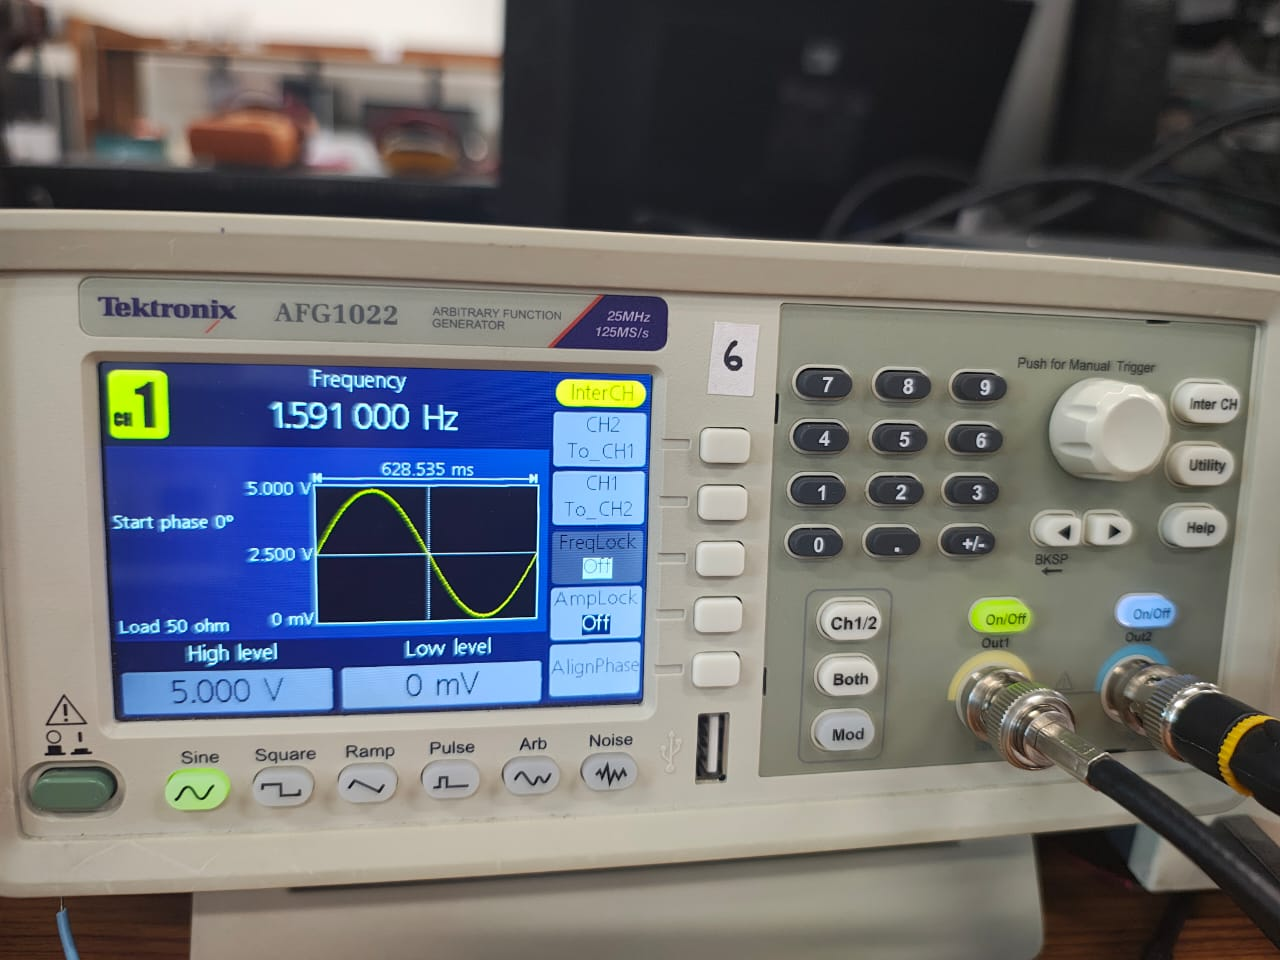
\includegraphics[width=\textwidth]{fig/1w10.jpeg} % Replace with actual file
        \caption{Function Generator Output for w = 10}
    \end{minipage}
\end{figure}

\subsubsection{w = 100}
\begin{figure}[H]
    \centering
    \begin{minipage}{0.48\textwidth}
        \centering
        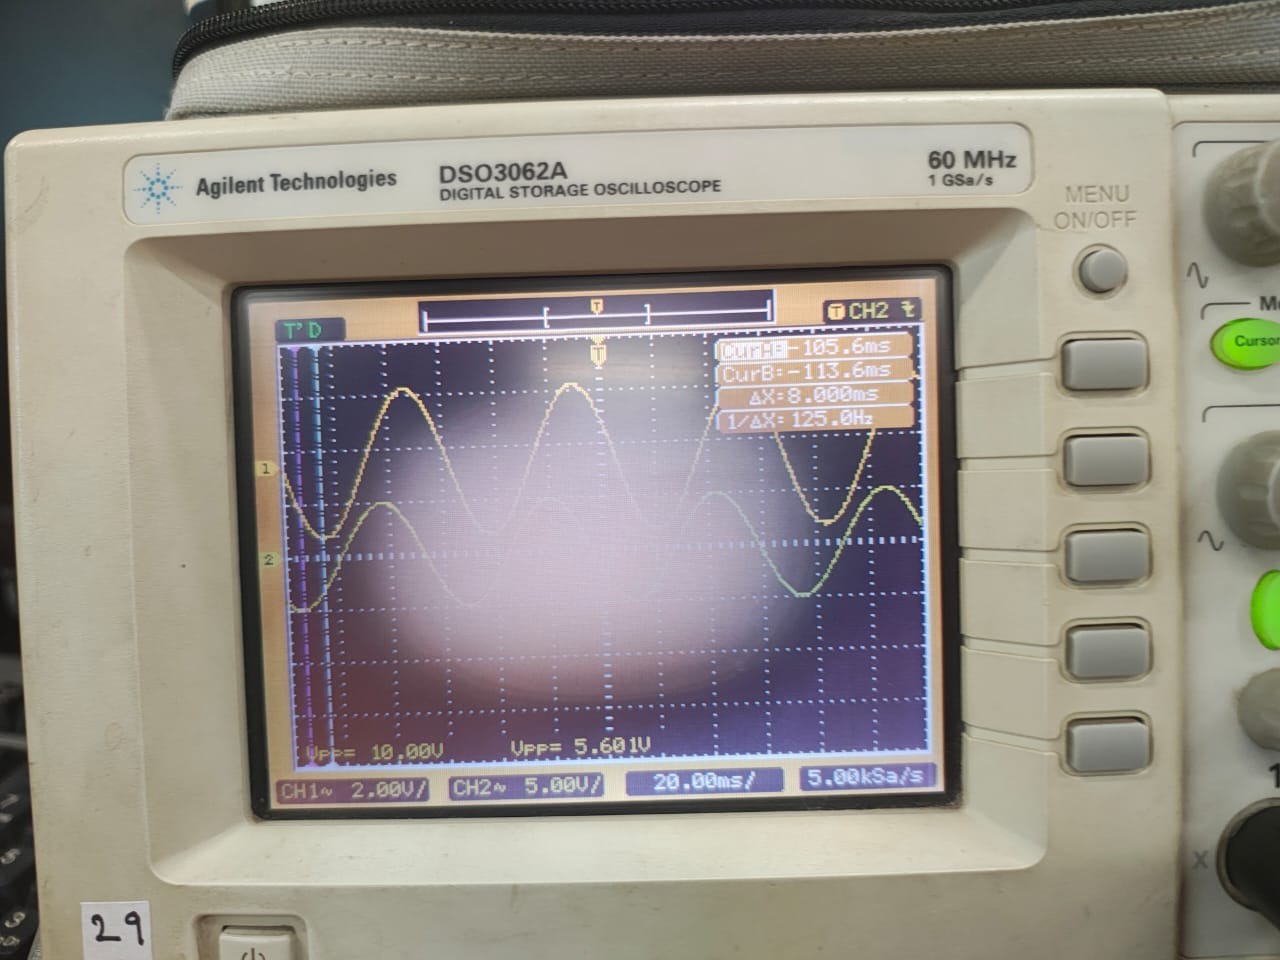
\includegraphics[width=\textwidth]{fig/1w100o.jpeg} % Replace with actual file
        \caption{Oscilloscope Reading for w = 100}
    \end{minipage}
    \hfill
    \begin{minipage}{0.48\textwidth}
        \centering
        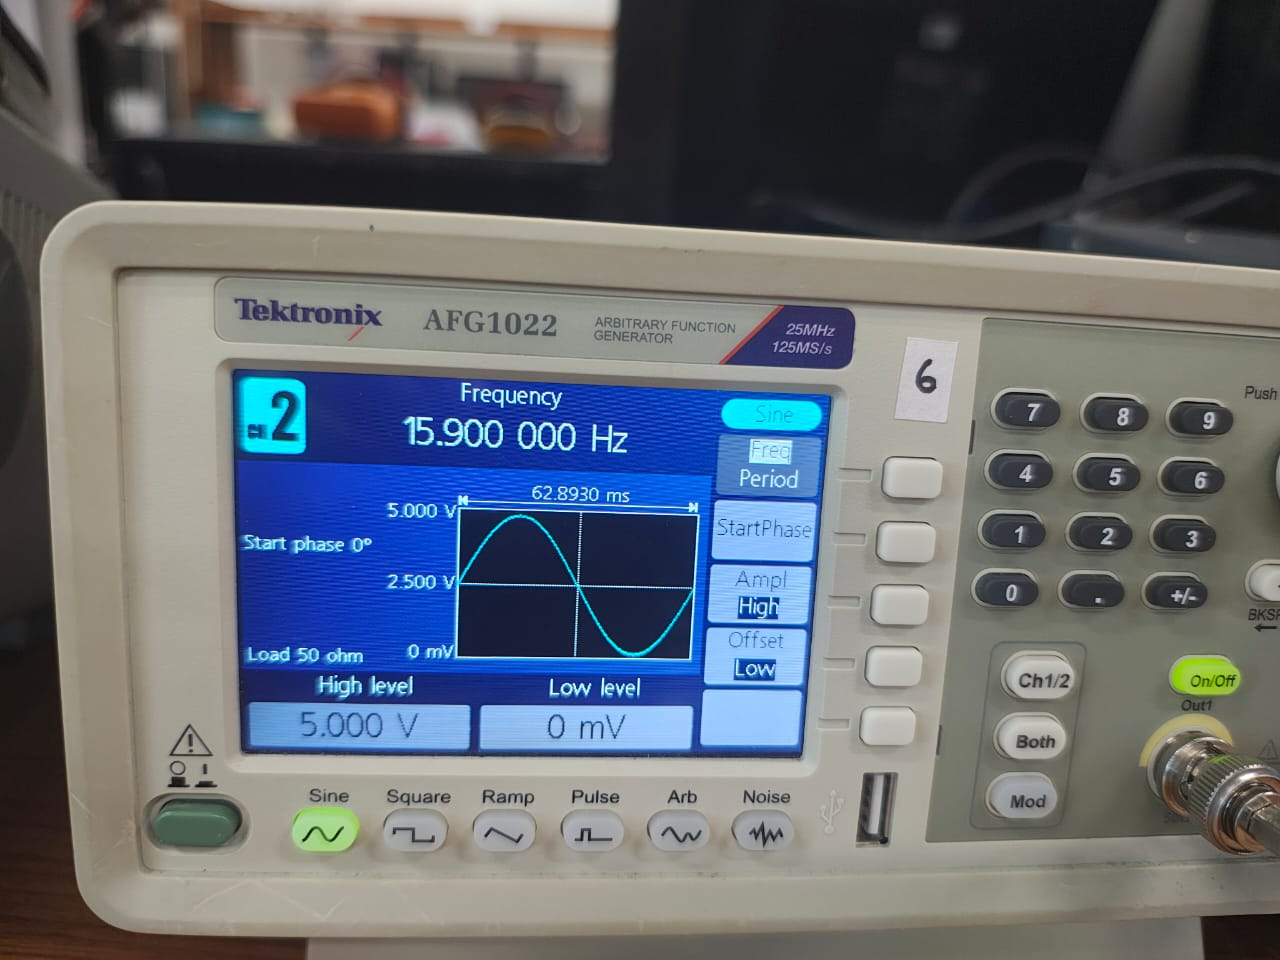
\includegraphics[width=\textwidth]{fig/1w100.jpeg} % Replace with actual file
        \caption{Function Generator Output for w = 100}
    \end{minipage}
\end{figure}

\subsubsection{w = 1000}
\begin{figure}[H]
    \centering
    \begin{minipage}{0.48\textwidth}
        \centering
        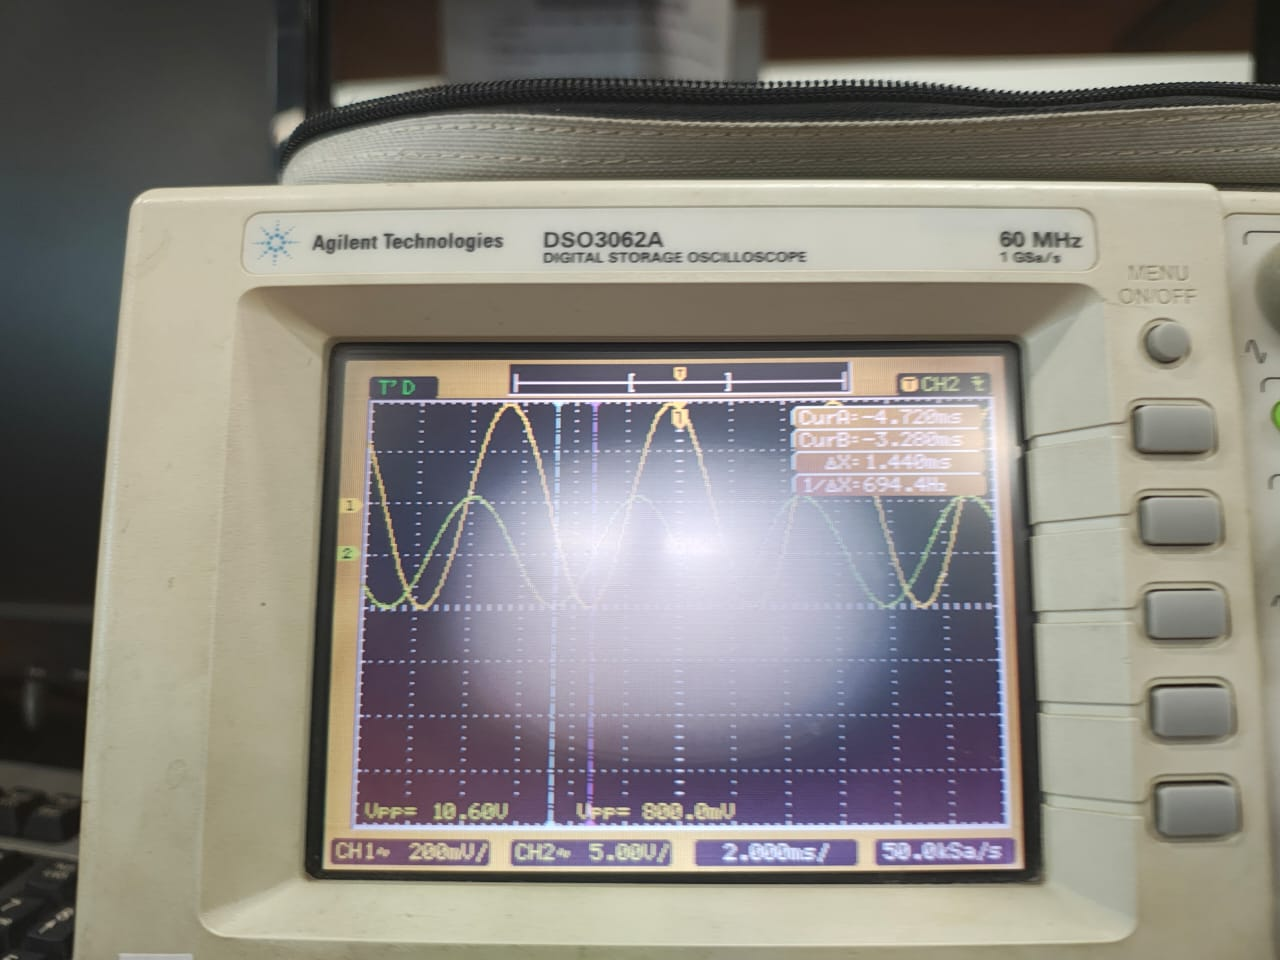
\includegraphics[width=\textwidth]{fig/1w1000o.jpeg} % Replace with actual file
        \caption{Oscilloscope Reading for w = 1000}
    \end{minipage}
    \hfill
    \begin{minipage}{0.48\textwidth}
        \centering
        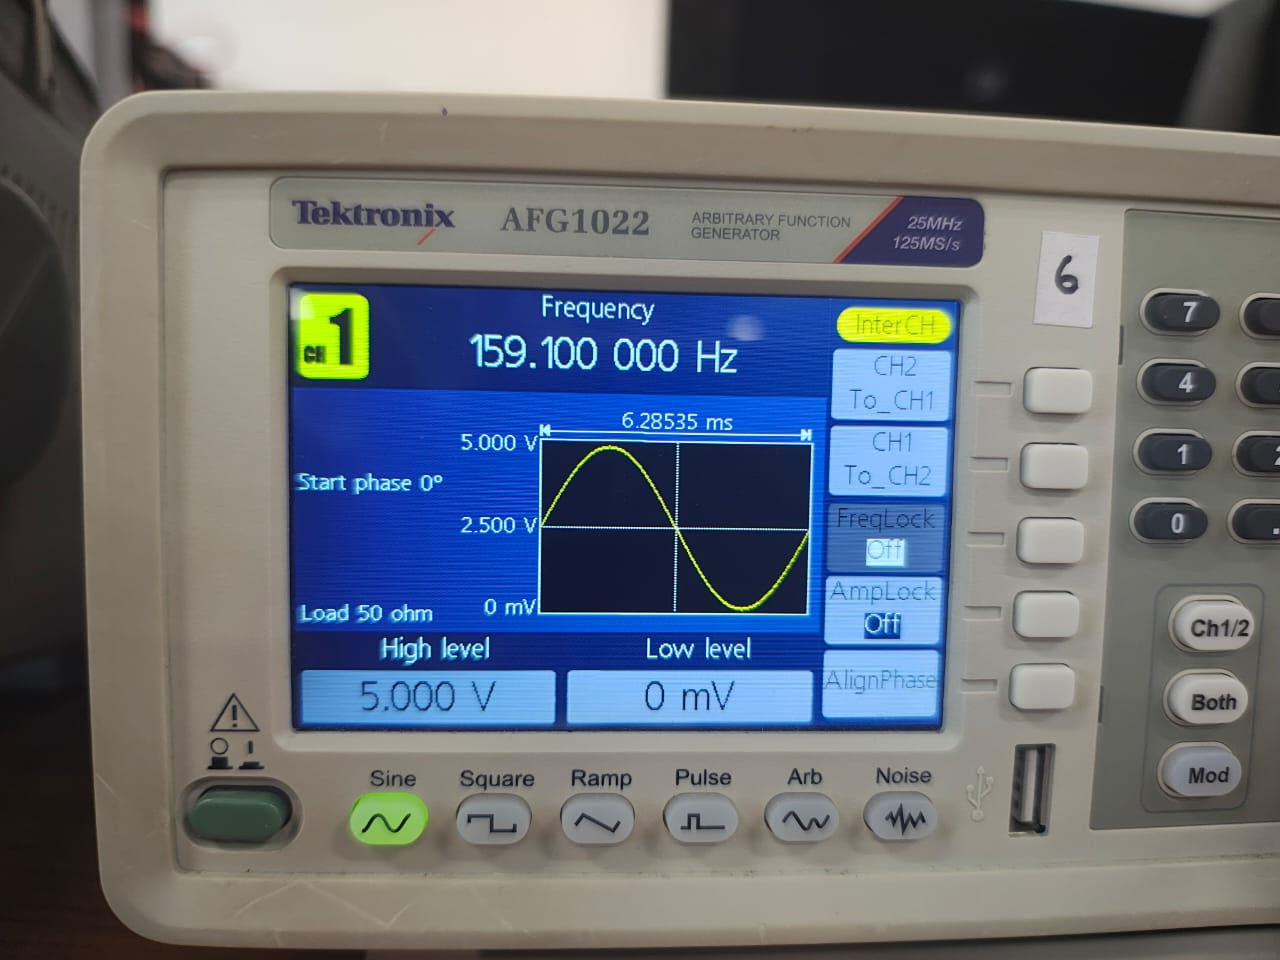
\includegraphics[width=\textwidth]{fig/1w1000.jpeg} % Replace with actual file
        \caption{Function Generator Output for w = 1000}
    \end{minipage}
\end{figure}
\subsection{Theoretical values}
\begin{align}
\phi &= -0.572^\circ , & \omega &= 10 \text{ rad/s} \\
\phi &= -5.7^\circ , & \omega &= 10 \text{ rad/s} \\
\phi &= -45^\circ , & \omega &= 100 \text{ rad/s} \\
\phi &= -84.29^\circ , & \omega &= 1000 \text{ rad/s}
\end{align}
\subsection{Magnitude Bode Plot}
\begin{figure}[H]
    \centering
    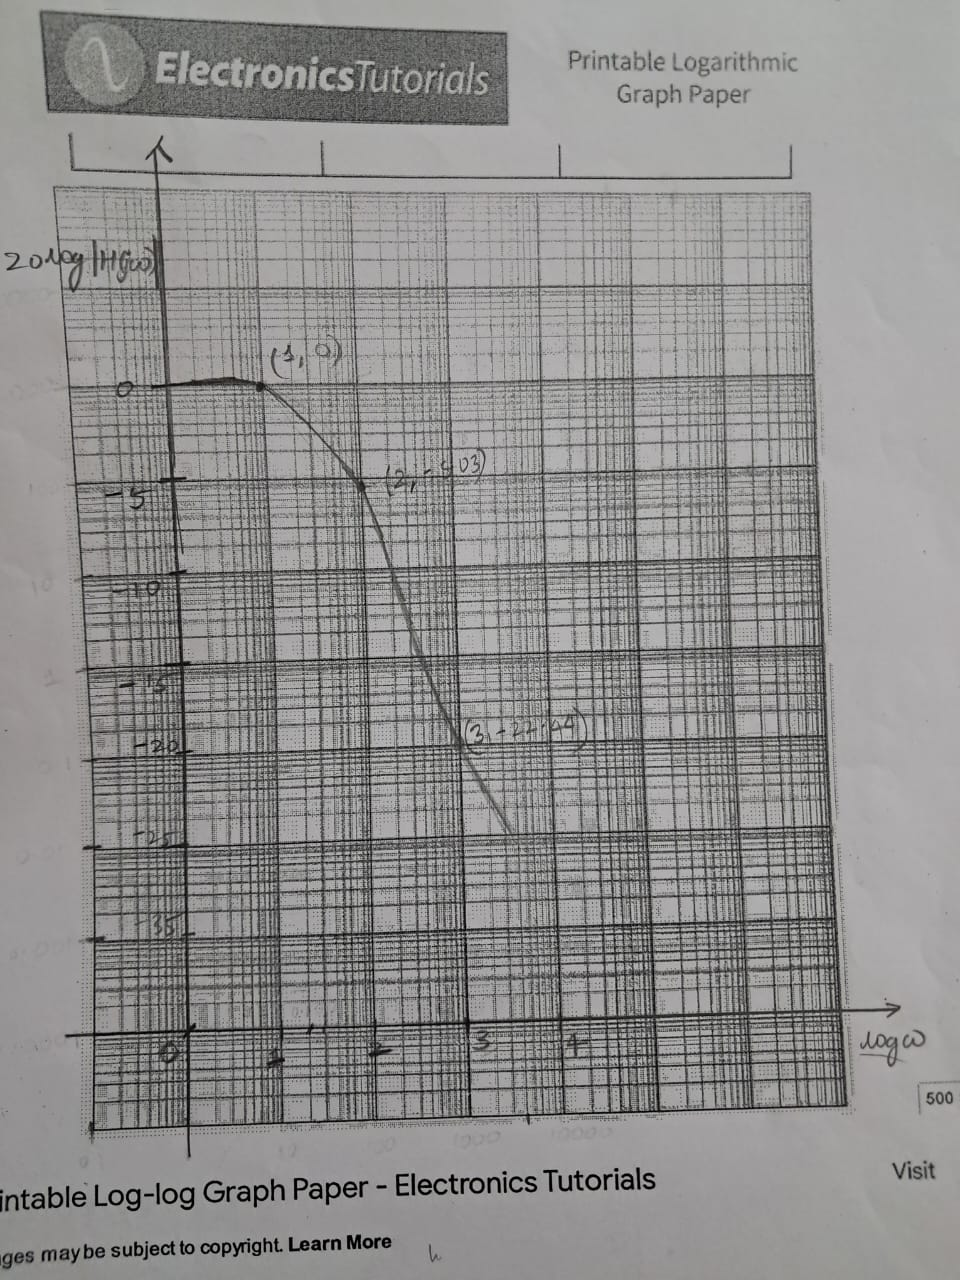
\includegraphics[width=0.7\textwidth]{fig/mbd1.jpeg} % Replace with actual file
    \caption{Magnitude Bode Plot for RC Circuit}
\end{figure}
Magnitude values(measured) are given by:
$$20\log{|H(j\omega)|}=20\log{V_{pp1}/V_{pp2}}$$
\begin{align}
20\log|H(j\omega)| &= 0.00 \text{ dB}, & \omega &= 10 \text{ rad/s} \\
20\log|H(j\omega)| &= -5.0362 \text{ dB}, & \omega &= 100 \text{ rad/s} \\
20\log|H(j\omega)| &= -22.4443 \text{ dB}, & \omega &= 1000 \text{ rad/s}
\end{align}
\subsection{Phase Bode Plot}
\begin{figure}[H]
    \centering
    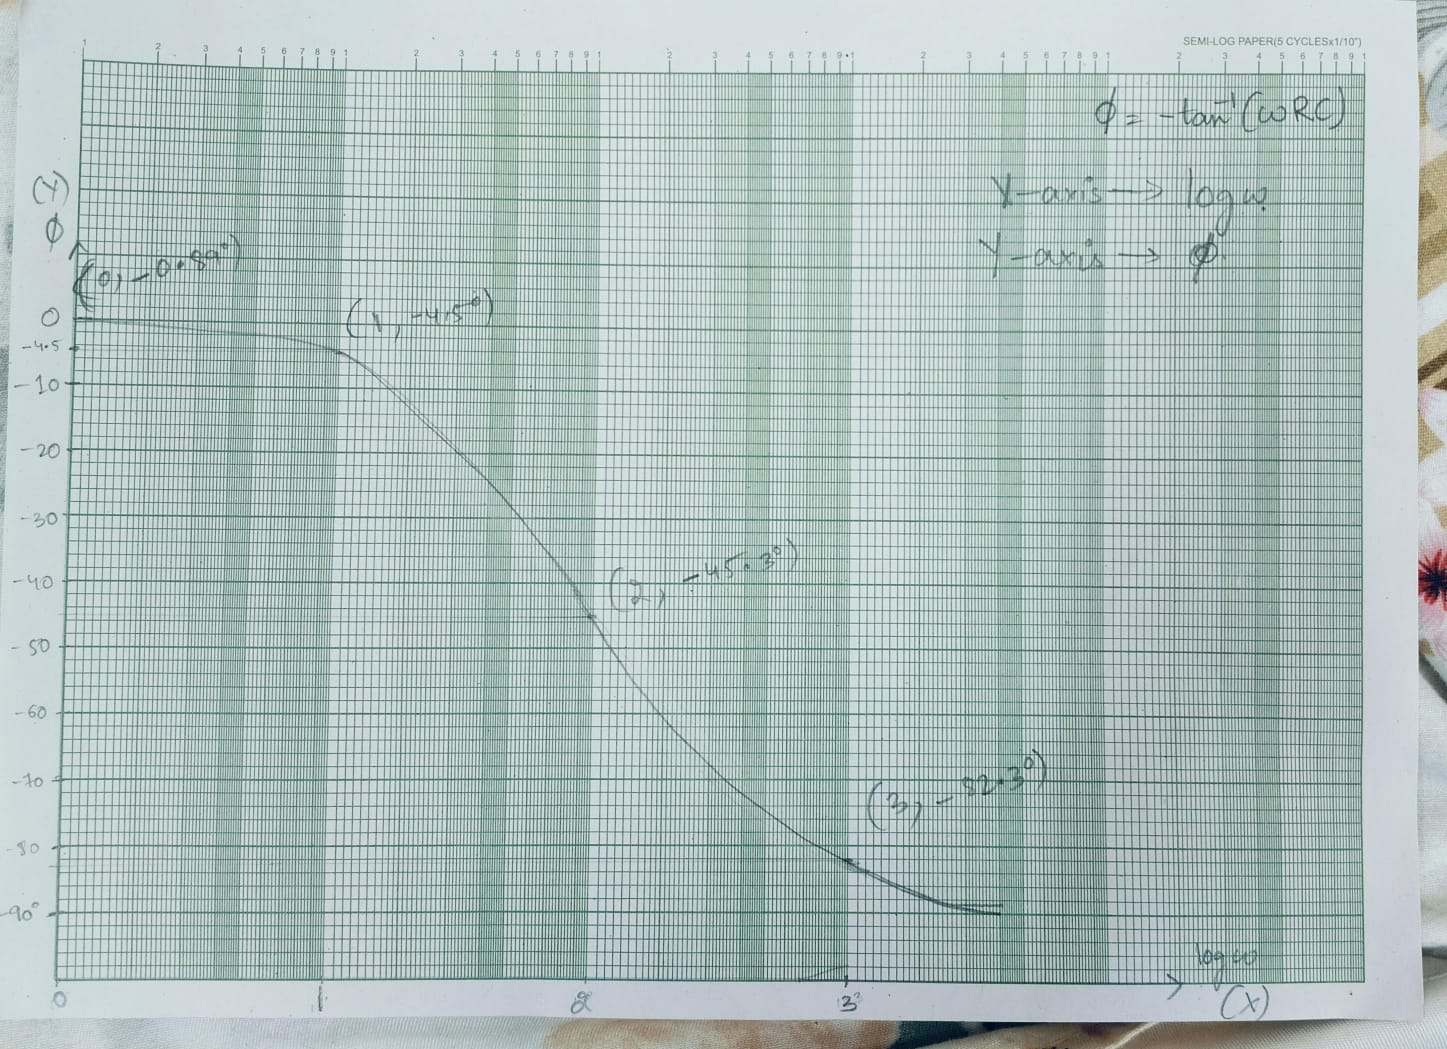
\includegraphics[width=0.7\textwidth]{fig/pbd1.jpeg} % Replace with actual file
    \caption{Phase Bode Plot for RC Circuit}
\end{figure}
Phase difference is given by:
$$\phi = \omega \times \delta t$$
\begin{align}
\phi &= -0.89^\circ, & \omega &= 1 \text{ rad/s} \\
\phi &= -4.5^\circ, & \omega &= 10 \text{ rad/s} \\
\phi &= -45.3^\circ, & \omega &= 100 \text{ rad/s} \\
\phi &= -82.3^\circ, & \omega &= 1000 \text{ rad/s}
\end{align}

\subsection{Case 2: Cascaded RC Circuit}
\subsubsection{Transfer Function}
Derived as:
\begin{equation}
    H(j\omega) = \frac{\frac{1}{2RC}}{ \frac{1-\omega^2R^2C^2}{2RC}+j\omega}
\end{equation}
Applying logarithm:
\begin{equation}
 \log(|H(j\omega)|)=-\log(2RC) -\frac{1}{2}(\log\frac{1-\omega^2R^2C^2}{2RC})^2+\omega^2)
\end{equation}
On simplification, we get:
\begin{equation}
20\log \left| H(j\omega) \right|=-40\log(RC) -20\log(\omega^2+\frac{1}{R^2C^2})
\end{equation}
For nth order circuit, we get 
\begin{equation}
    \phi = -n\tan^{-1}(RC\omega)
\end{equation}
We get phase to be :
\begin{equation}
    \phi =-2\tan^{-1}(RC\omega)
\end{equation}

\subsection{Oscilloscope- Practically measured VPP}
\subsubsection{w = 10}
\begin{figure}[H]
    \centering
    \begin{minipage}{0.48\textwidth}
        \centering
        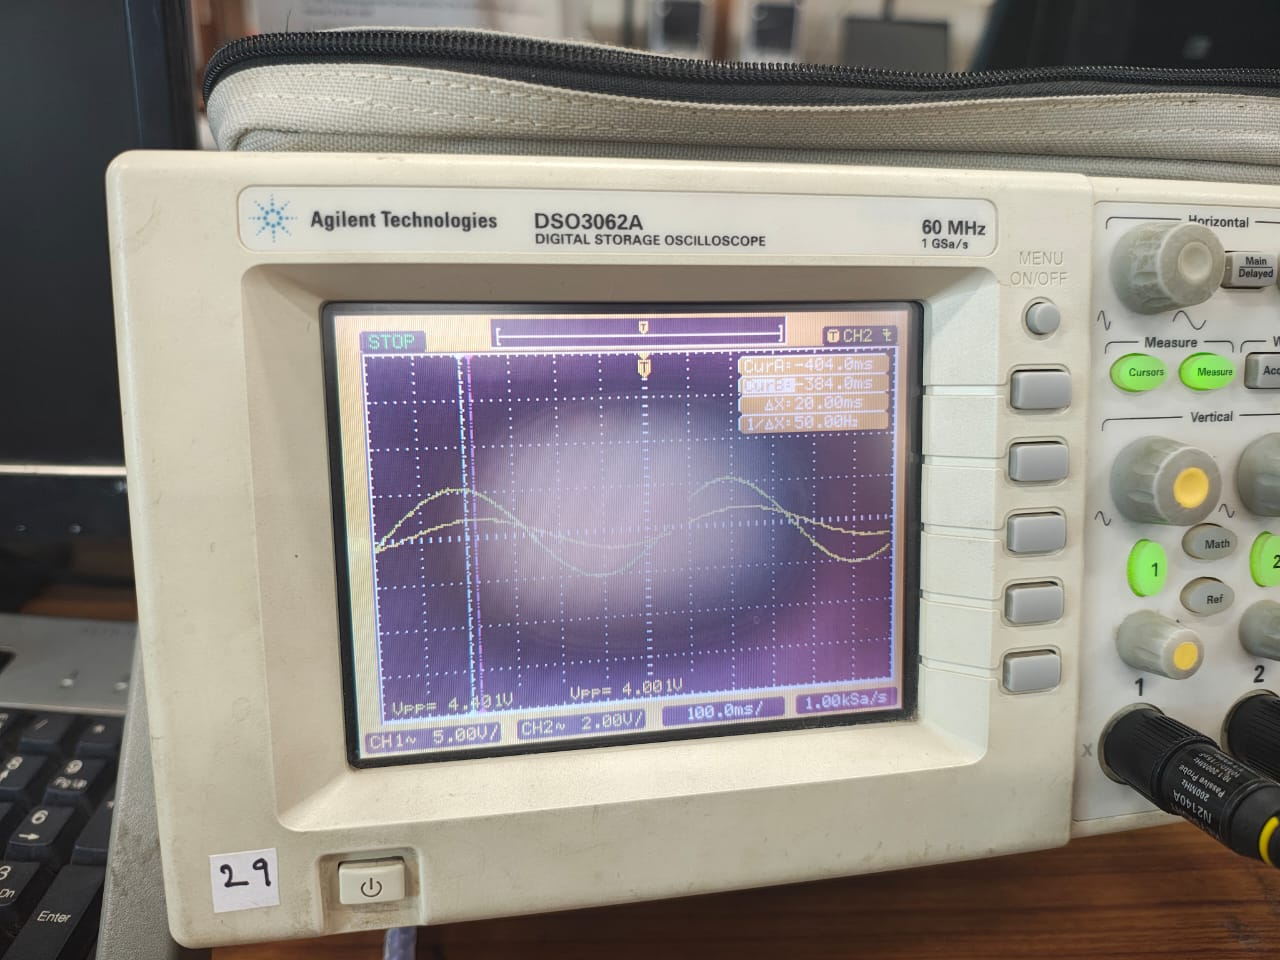
\includegraphics[width=\textwidth]{fig/2w10o.jpeg} % Replace with actual file
        \caption{Oscilloscope Reading for w = 10}
    \end{minipage}
    \hfill
    \begin{minipage}{0.48\textwidth}
        \centering
        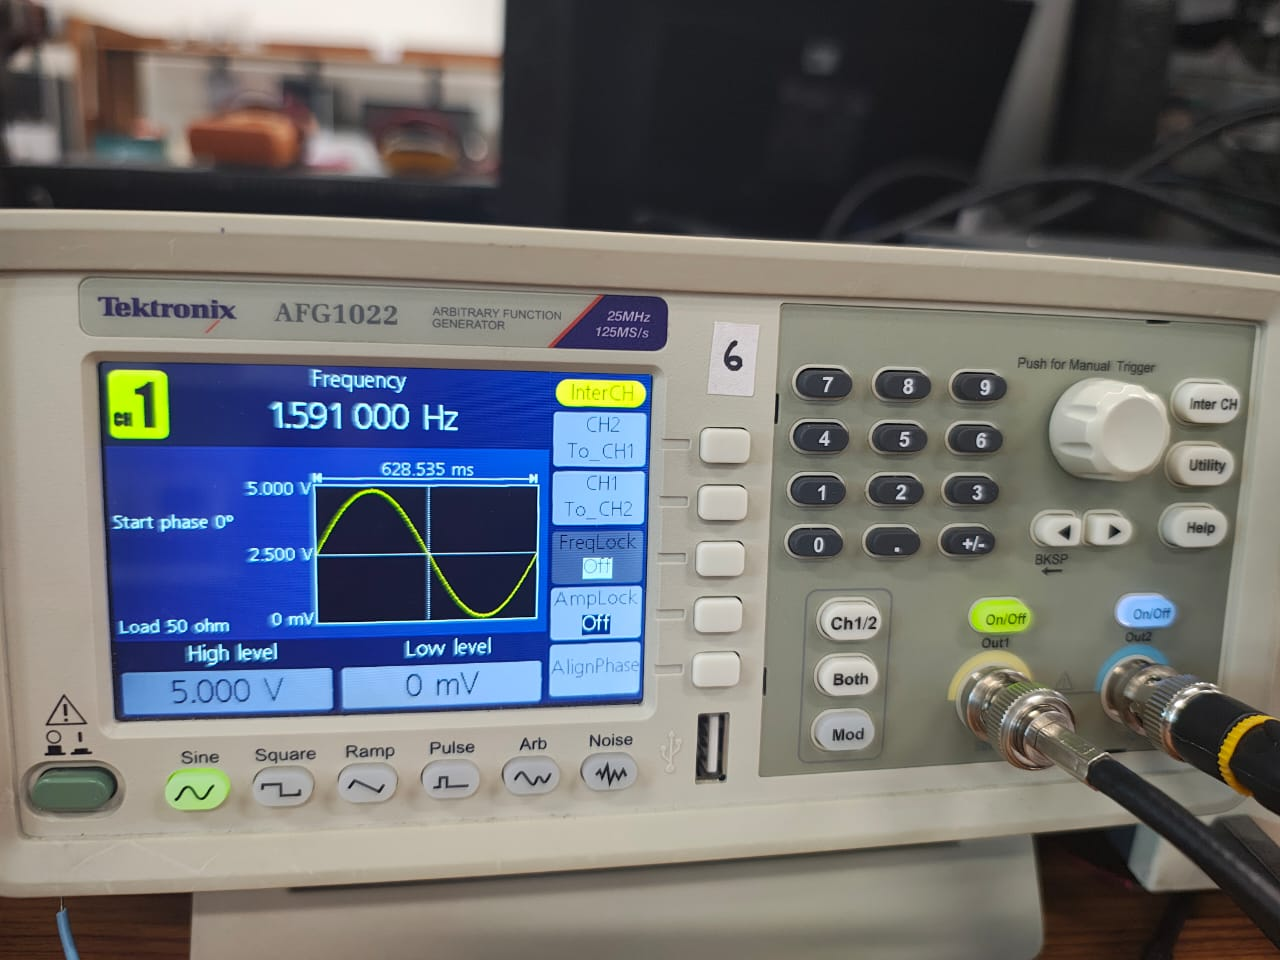
\includegraphics[width=\textwidth]{fig/2w10.jpeg} % Replace with actual file
        \caption{Function Generator Output for w = 10}
    \end{minipage}
\end{figure}

\subsubsection{w = 100}
\begin{figure}[H]
    \centering
    \begin{minipage}{0.48\textwidth}
        \centering
        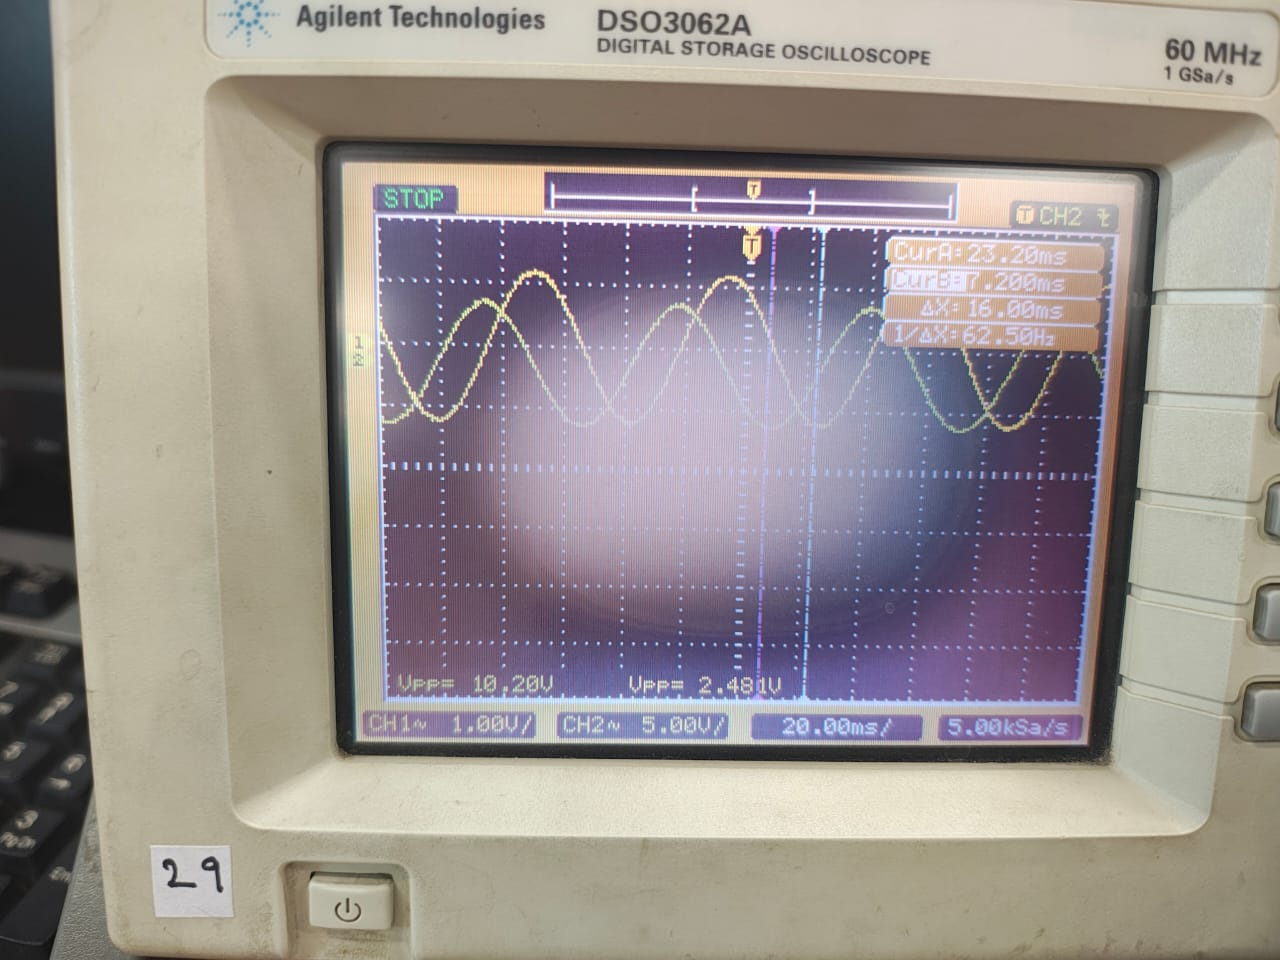
\includegraphics[width=\textwidth]{fig/2w100o.jpeg} % Replace with actual file
        \caption{Oscilloscope Reading for w = 100}
    \end{minipage}
    \hfill
    \begin{minipage}{0.48\textwidth}
        \centering
        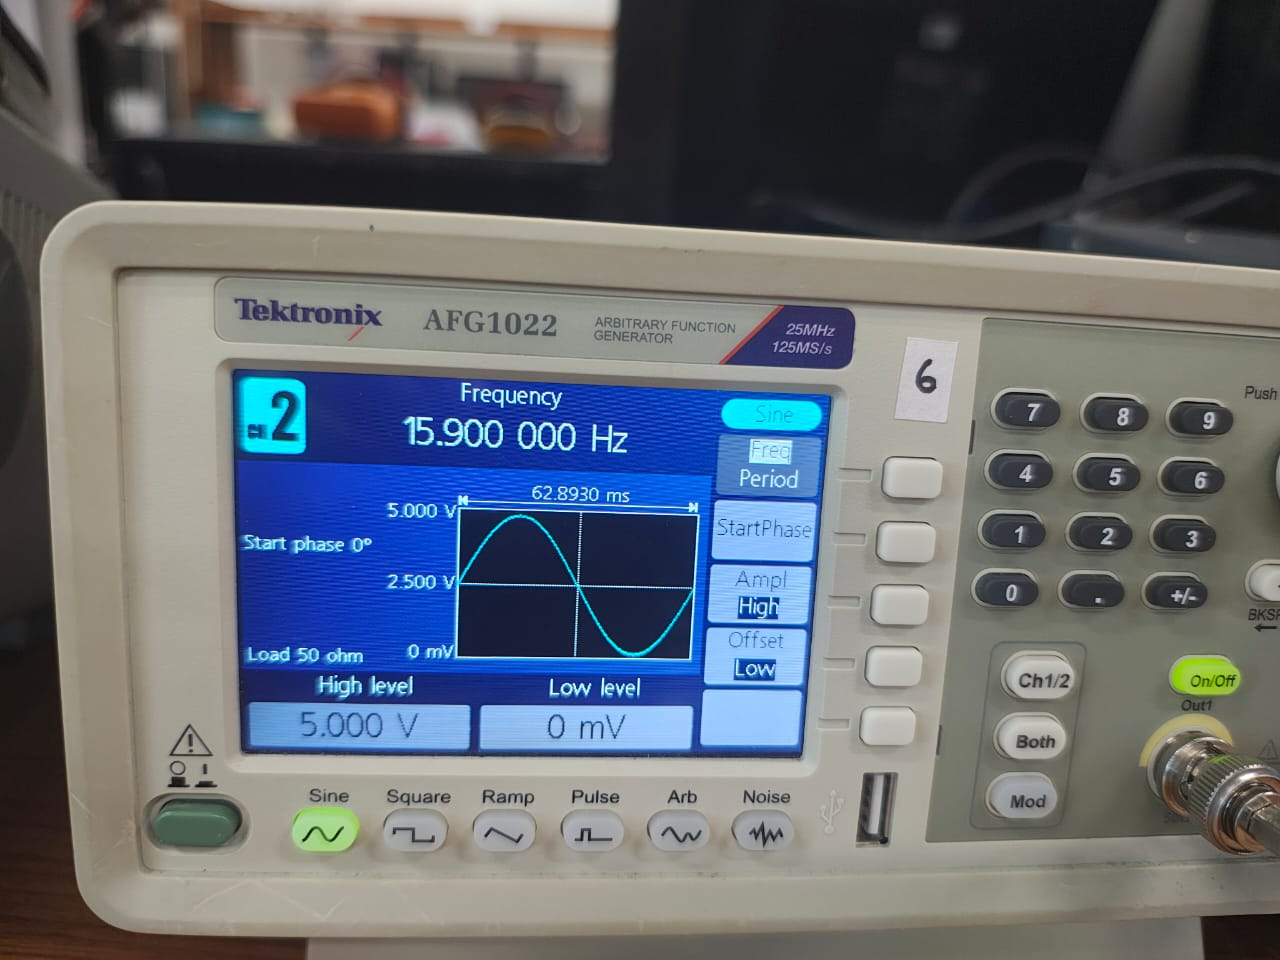
\includegraphics[width=\textwidth]{fig/1w100.jpeg} % Replace with actual file
        \caption{Function Generator Output for w = 100}
    \end{minipage}
\end{figure}

\subsubsection{w = 1000}
\begin{figure}[H]
    \centering
    \begin{minipage}{0.48\textwidth}
        \centering
        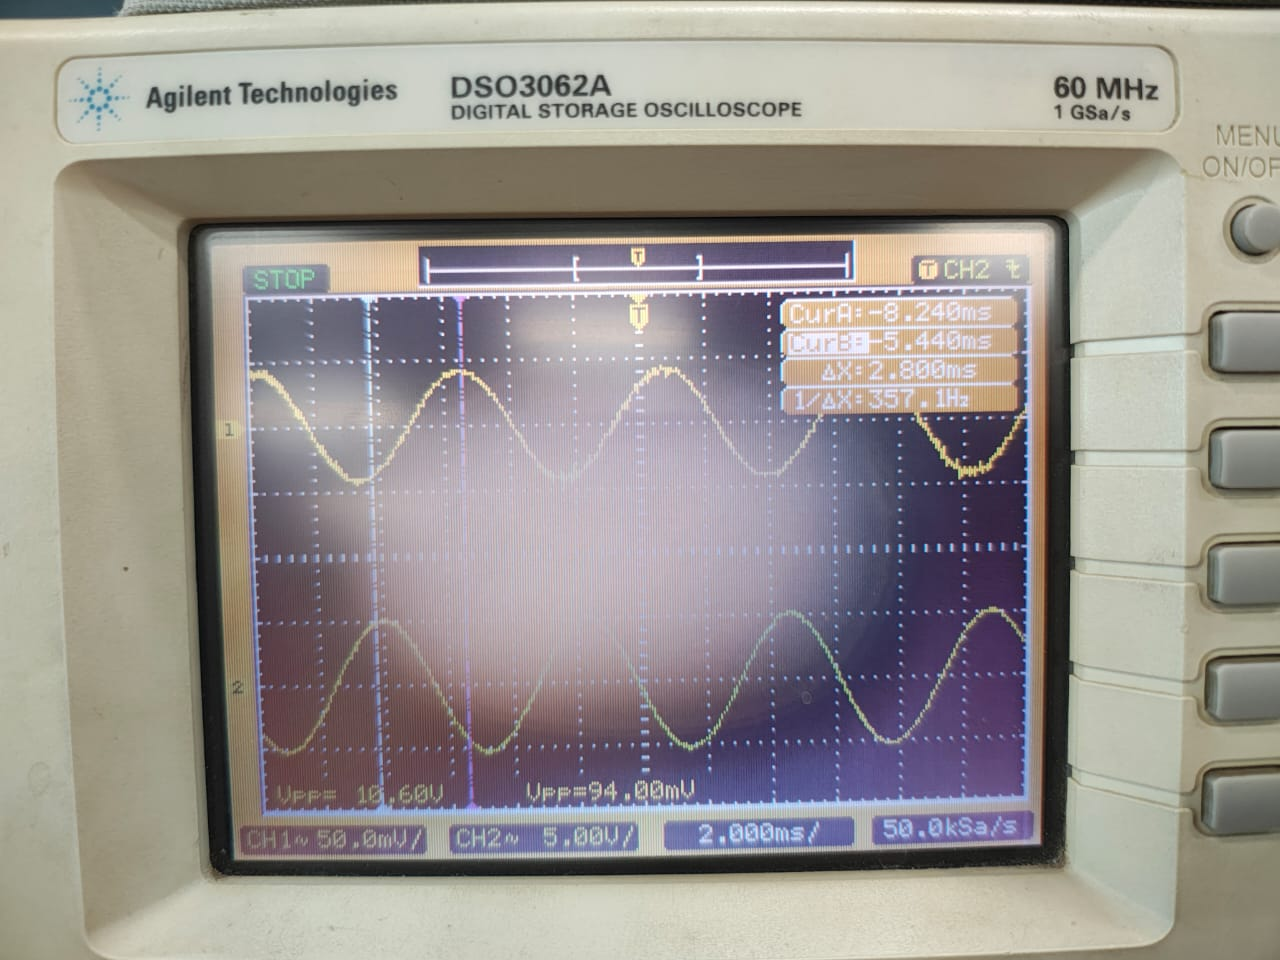
\includegraphics[width=\textwidth]{fig/2w1000o.jpeg} % Replace with actual file
        \caption{Oscilloscope Reading for w = 1000}
    \end{minipage}
    \hfill
    \begin{minipage}{0.48\textwidth}
        \centering
        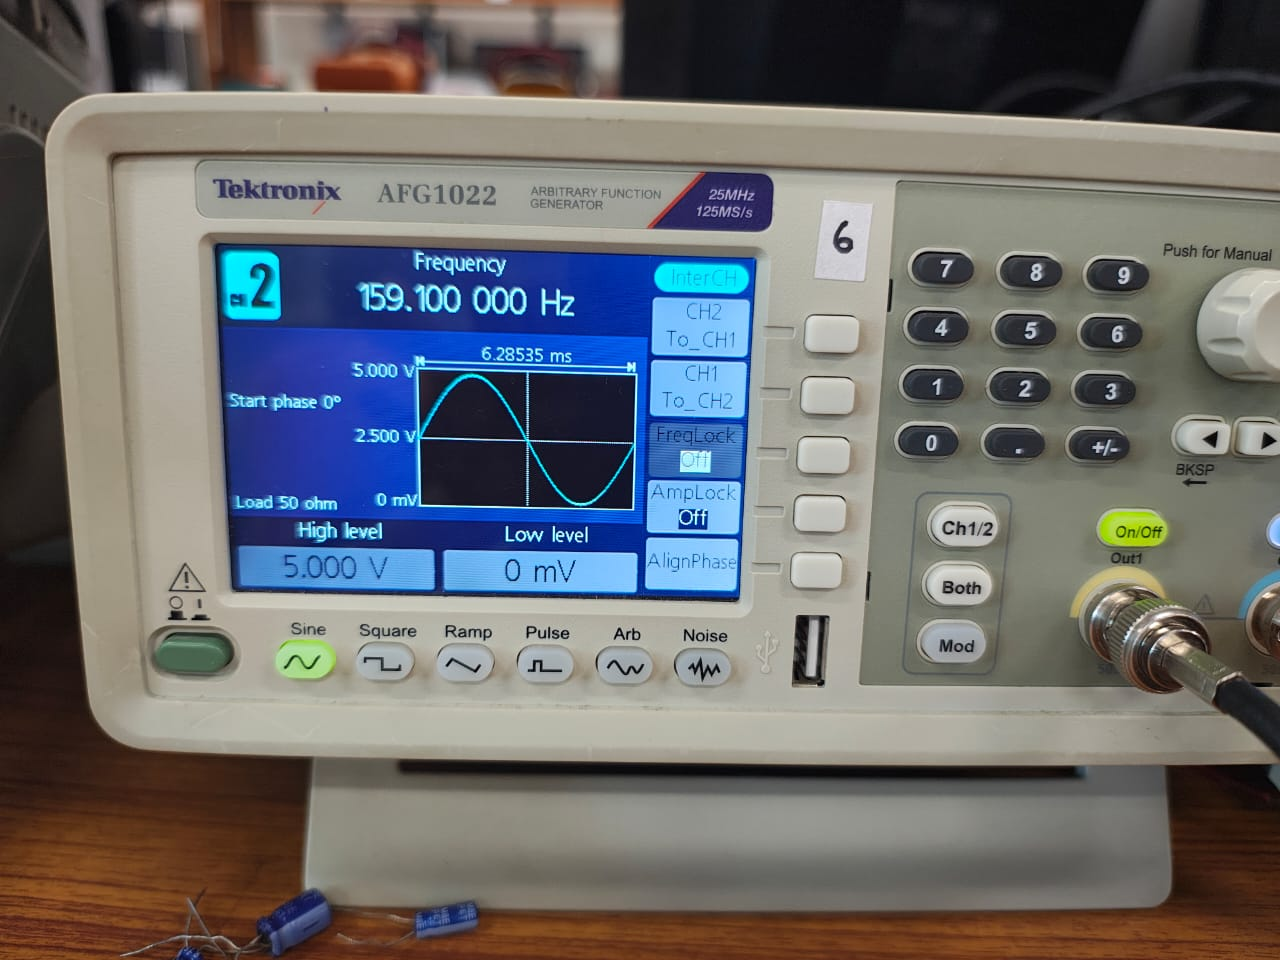
\includegraphics[width=\textwidth]{fig/2w1000.jpeg} % Replace with actual file
        \caption{Function Generator Output for w = 1000}
    \end{minipage}
\end{figure}
\subsection{Theoretical values}
\begin{align}
\phi &= -11.4^\circ , & \omega &= 10 \text{ rad/s} \\
\phi &= -90^\circ , & \omega &= 100 \text{ rad/s} \\
\phi &= -168.58^\circ , & \omega &= 1000 \text{ rad/s}
\end{align}
\subsection{Magnitude Bode Plot}
\begin{figure}[H]
    \centering
    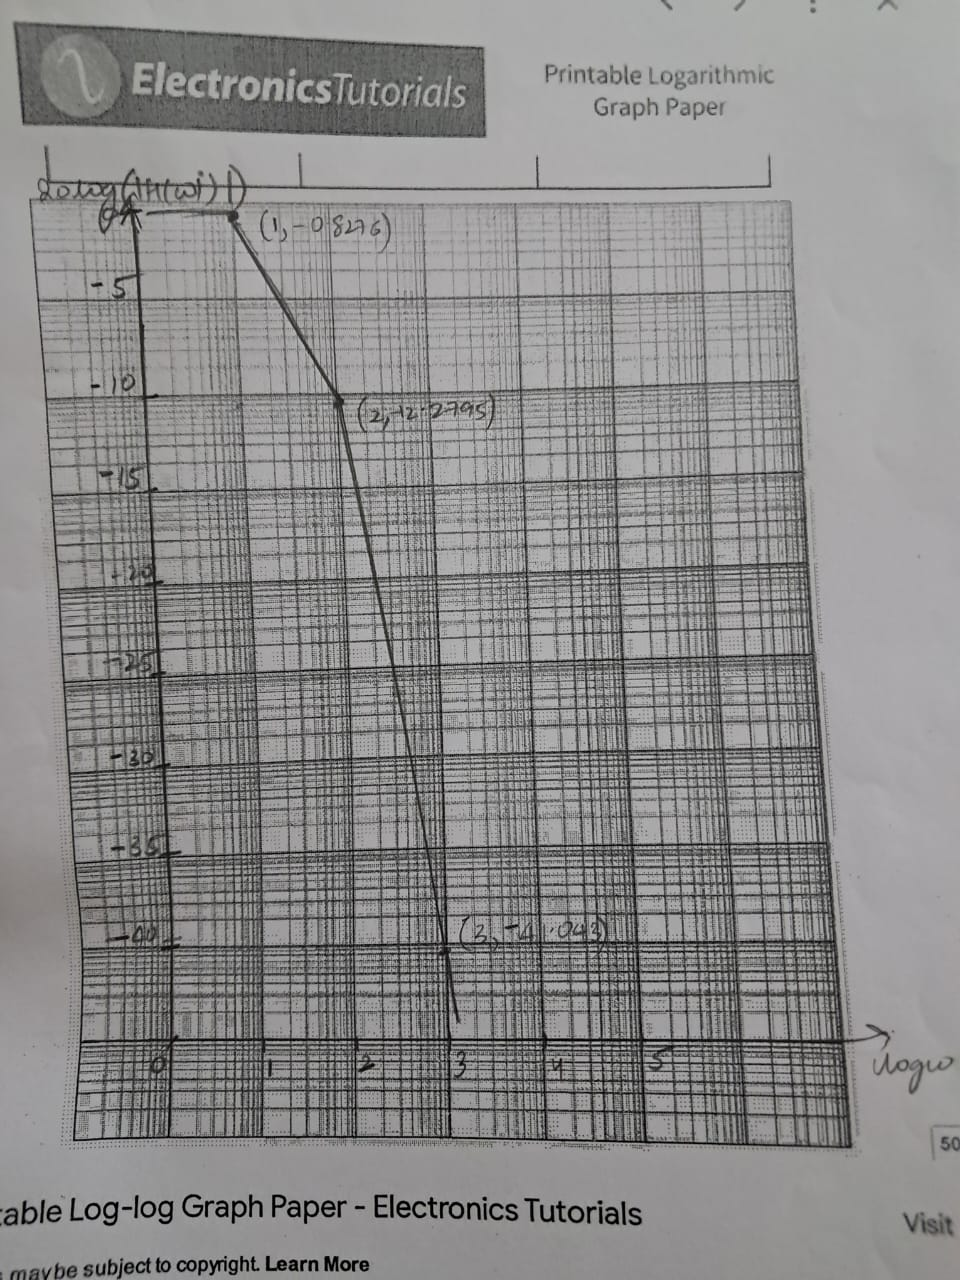
\includegraphics[width=0.7\textwidth]{fig/mbd2.jpeg} % Replace with actual file
    \caption{Magnitude Bode Plot for RC Circuit}
\end{figure}
Magnitude values(measured) are given by:
$$20\log{|H(j\omega)|}=20\log{V_{pp1}/V_{pp2}}$$
\begin{align}
20\log|H(j\omega)| &= -0.8276 \text{ dB}, & \omega &= 10 \text{ rad/s} \\
20\log|H(j\omega)| &= -12.2795 \text{ dB}, & \omega &= 100 \text{ rad/s} \\
20\log|H(j\omega)| &= -41.043 \text{ dB}, & \omega &= 1000 \text{ rad/s}
\end{align}
\subsection{Phase Bode Plot}
\begin{figure}[H]
    \centering
    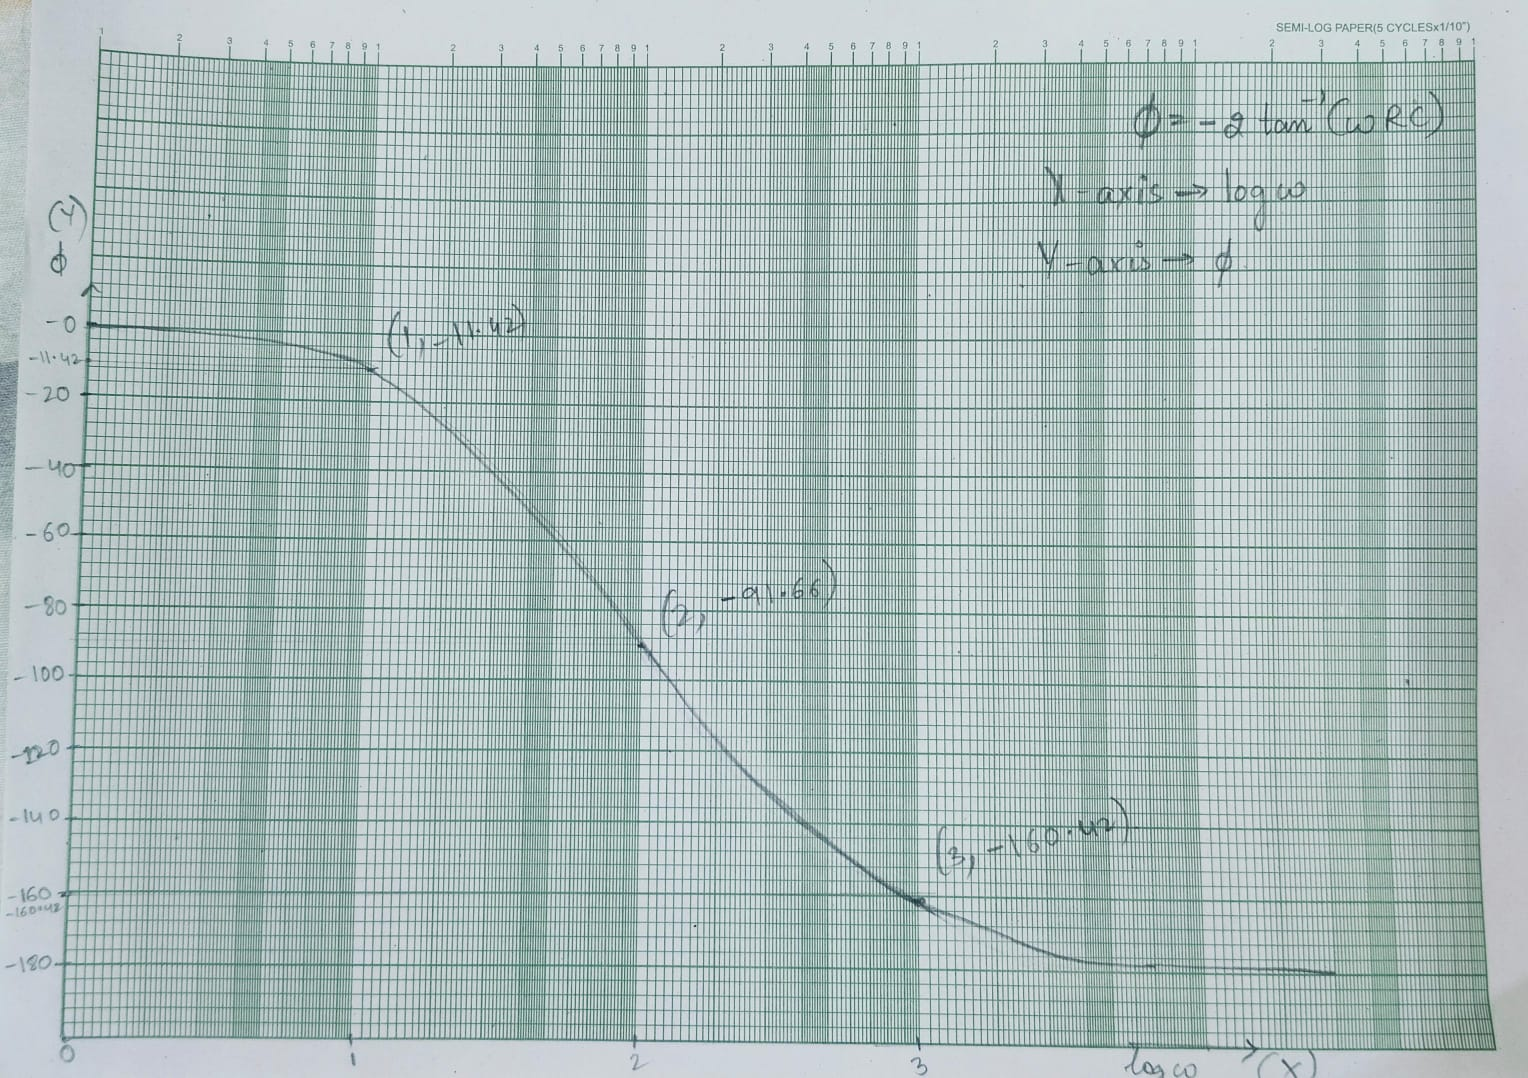
\includegraphics[width=0.7\textwidth]{fig/pbd2.jpeg} % Replace with actual file
    \caption{Phase Bode Plot for RC Circuit}
\end{figure}
Phase difference is given by:
$$\phi = \omega \times \delta t$$
\begin{align}
\phi &= -11.42^\circ, & \omega &= 10 \text{ rad/s} \\
\phi &= --91.66^\circ, & \omega &= 100 \text{ rad/s} \\
\phi &= -160.42^\circ, & \omega &= 1000 \text{ rad/s}
\end{align}


\subsection{Case 3: Twice-Cascaded RC Circuit}
\subsubsection{Circuit Diagram}
\begin{figure}[H]
    \centering
    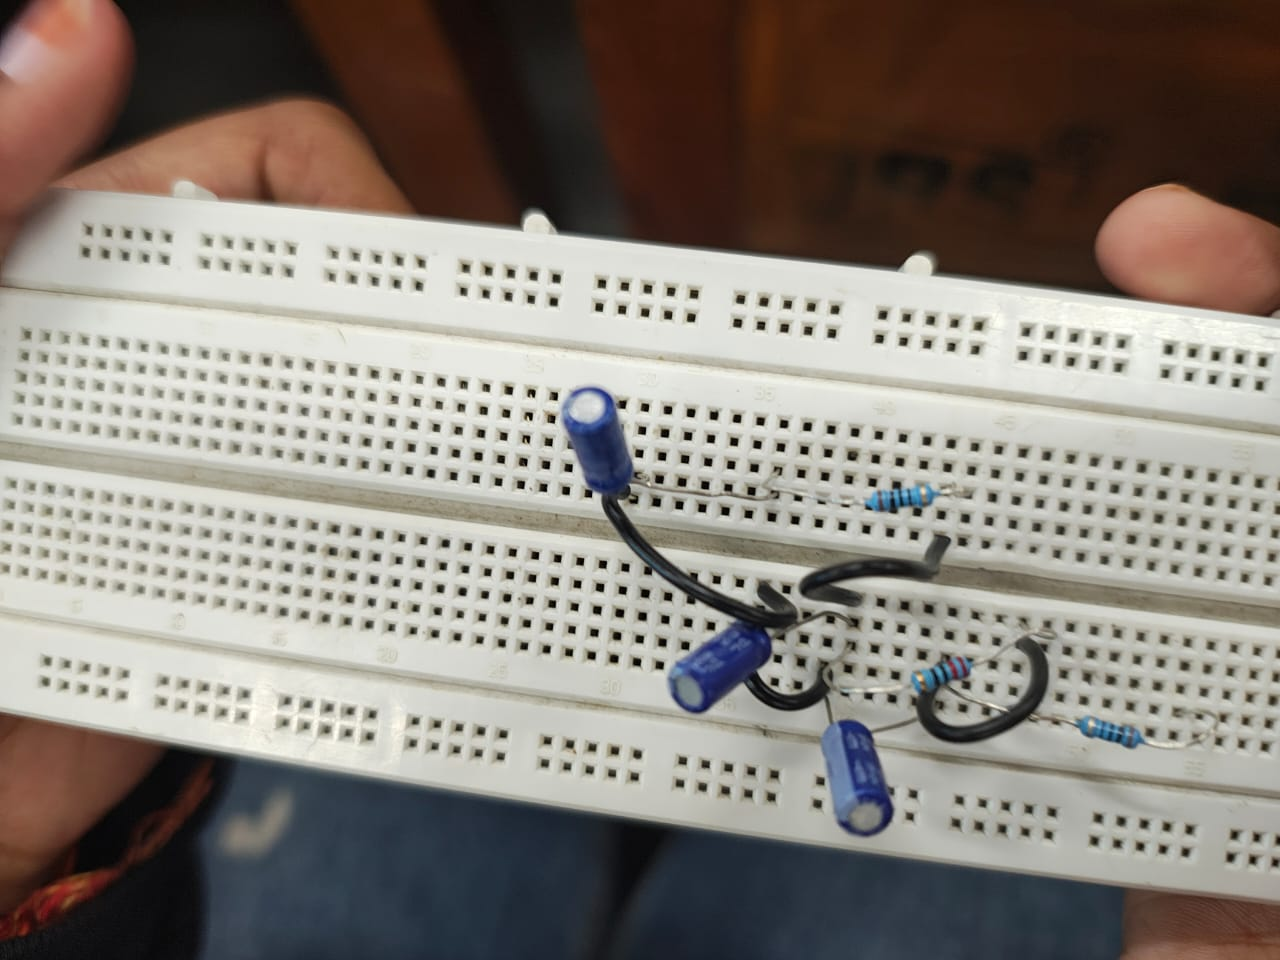
\includegraphics[width=0.7\textwidth]{fig/rc3.jpeg} % Replace with actual file
    \caption{RC Circuit Diagram}
\end{figure}

\subsubsection{Transfer Function}
Derived as:
\begin{equation}
    H(s) = \frac{\frac{1}{3RC+s^2R^3C^3}}{(\frac{1+3s^2R^2C^2}{3RC+s^2R^3C^3}+s)}
\end{equation}
Since $s=j\omega$
\begin{equation}
    H(j\omega) = \frac{\frac{1}{3RC-\omega^2R^3C^3}}{\frac{1-3\omega^2R^2C^2}{3RC-\omega^2R^3C^3}+j\omega}
\end{equation}
Applying logarithm:
\begin{equation}
\log \left| H(s) \right| = -\log \left( 3RC - \omega^2 R^3 C^3 \right) - \frac{1}{2} \log \left( \left( \frac{1 - 3\omega^2 R^2 C^2}{3RC - \omega^2 R^3 C^3} \right)^2 + \omega^2 \right)
\end{equation}
On simplification, we get:
\begin{equation}
\log \left| H(s) \right|=-\frac{3}{2} \left( 2\log (RC) + \log \left( \omega^2 + \frac{1}{R^2C^2} \right) \right)
\end{equation}
\begin{equation}
    20\log \left| H(s) \right|=-30 \left( 2\log (RC) + \log \left( \omega^2 + \frac{1}{R^2C^2} \right) \right)
\end{equation}
For nth order circuit, we get 
\begin{equation}
    \phi = -n\tan^{-1}(RC\omega)
\end{equation}
We get phase to be :
\begin{equation}
    \phi =-3\tan^{-1}(RC\omega)
\end{equation}

\subsection{Oscilloscope - Practically Measured VPP's}


\subsubsection{w = 10}
\begin{figure}[H]
    \centering
    \begin{minipage}{0.48\textwidth}
        \centering
        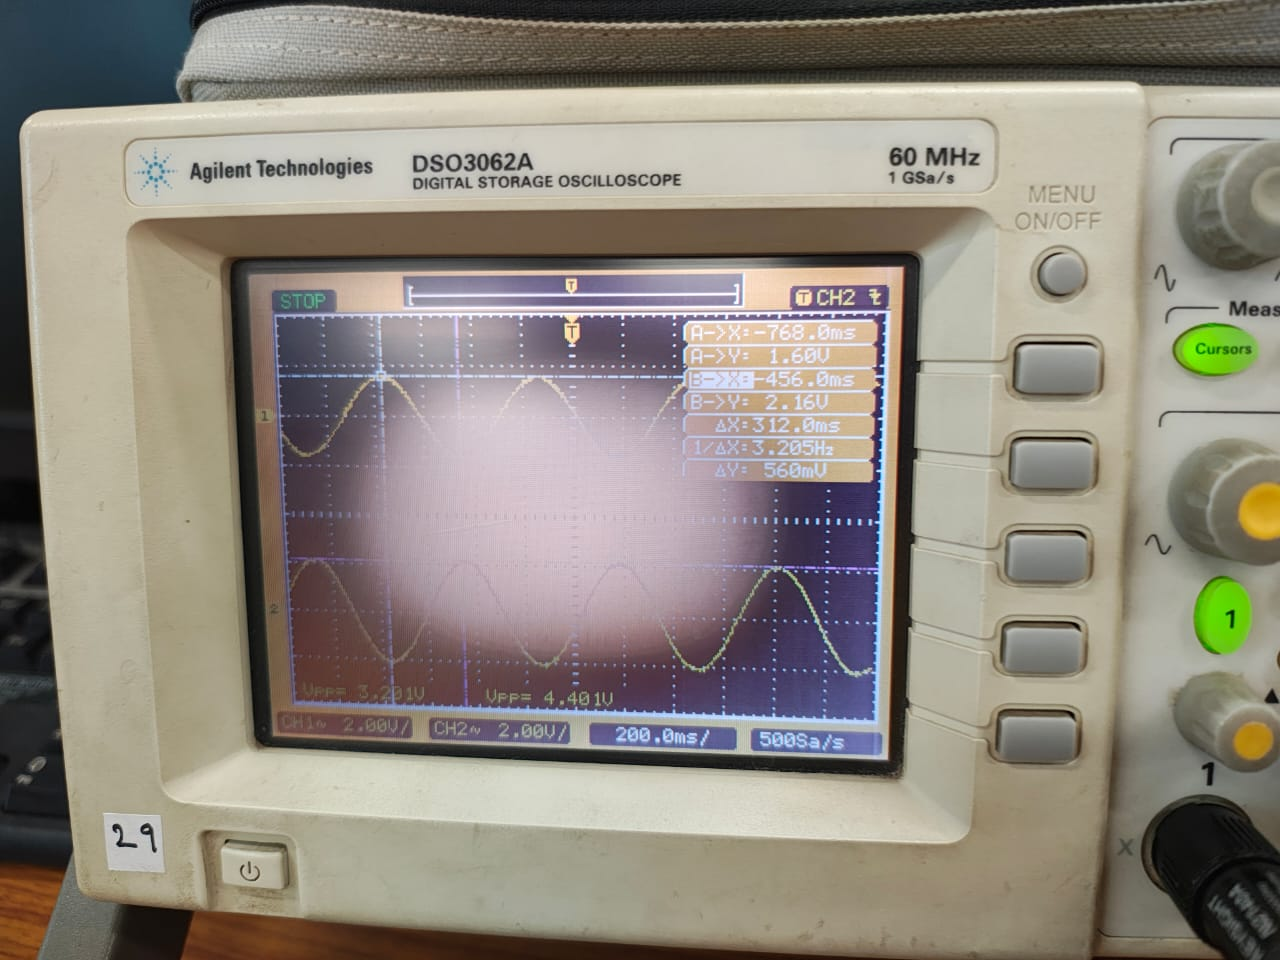
\includegraphics[width=\textwidth]{fig/3w10o.jpeg} % Replace with actual file
        \caption{Oscilloscope Reading for w = 10}
    \end{minipage}
    \hfill
    \begin{minipage}{0.48\textwidth}
        \centering
        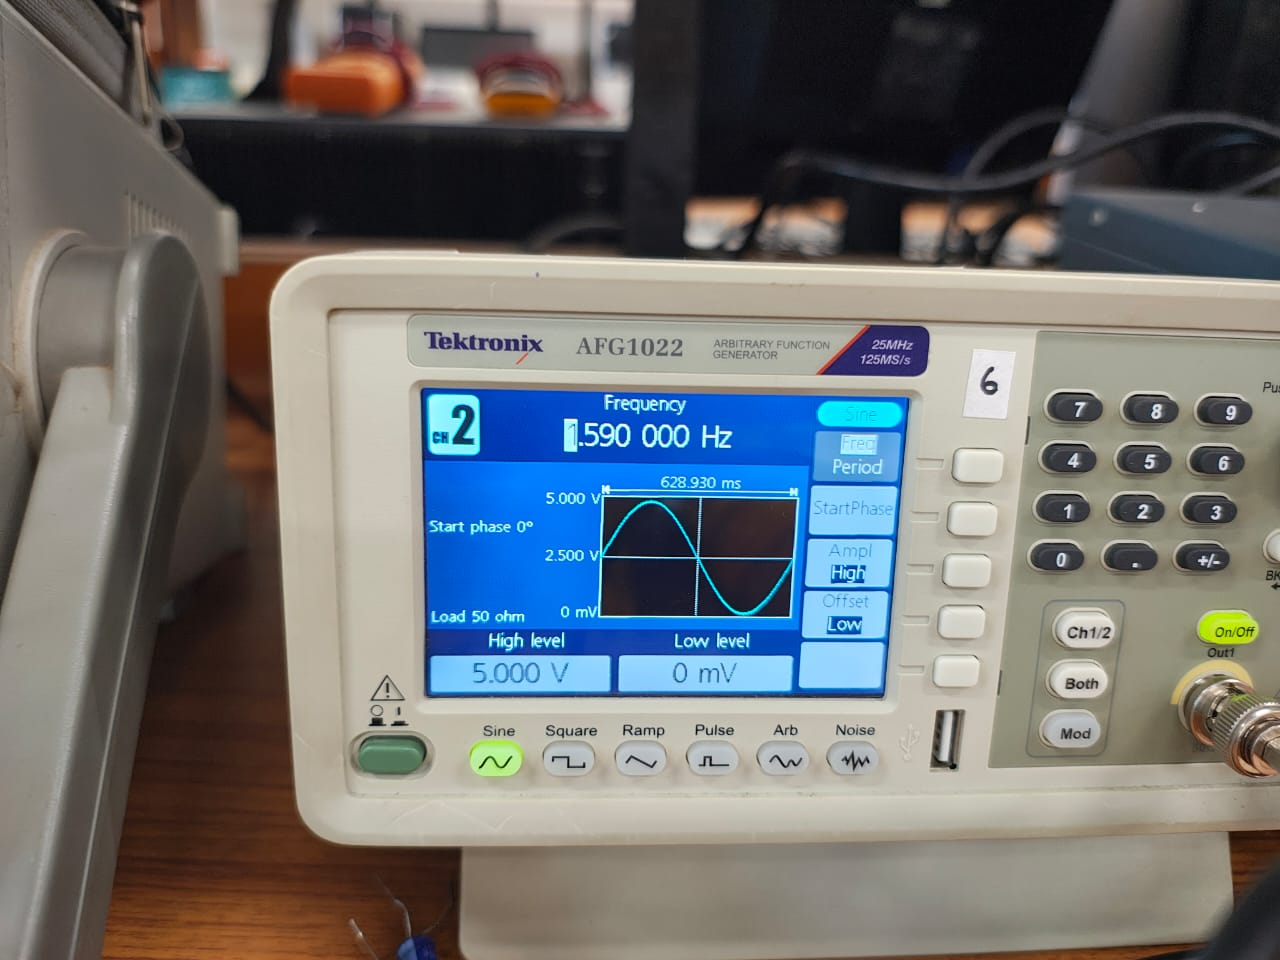
\includegraphics[width=\textwidth]{fig/3w10.jpeg} % Replace with actual file
        \caption{Function Generator Output for w = 10}
    \end{minipage}
\end{figure}

\subsubsection{w = 100}
\begin{figure}[H]
    \centering
    \begin{minipage}{0.48\textwidth}
        \centering
        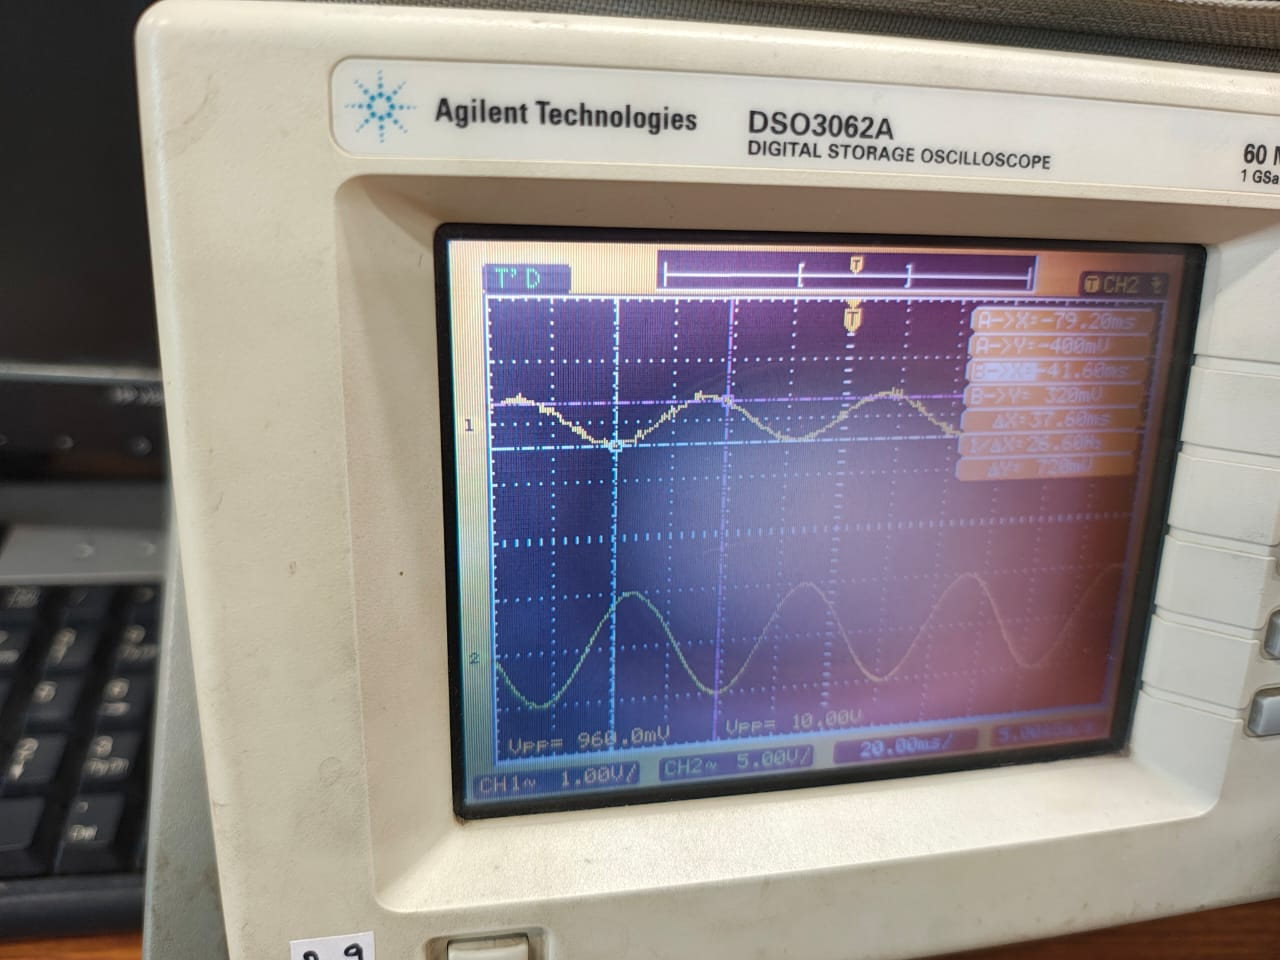
\includegraphics[width=\textwidth]{fig/3w100o.jpeg} % Replace with actual file
        \caption{Oscilloscope Reading for w = 100}
    \end{minipage}
    \hfill
    \begin{minipage}{0.48\textwidth}
        \centering
        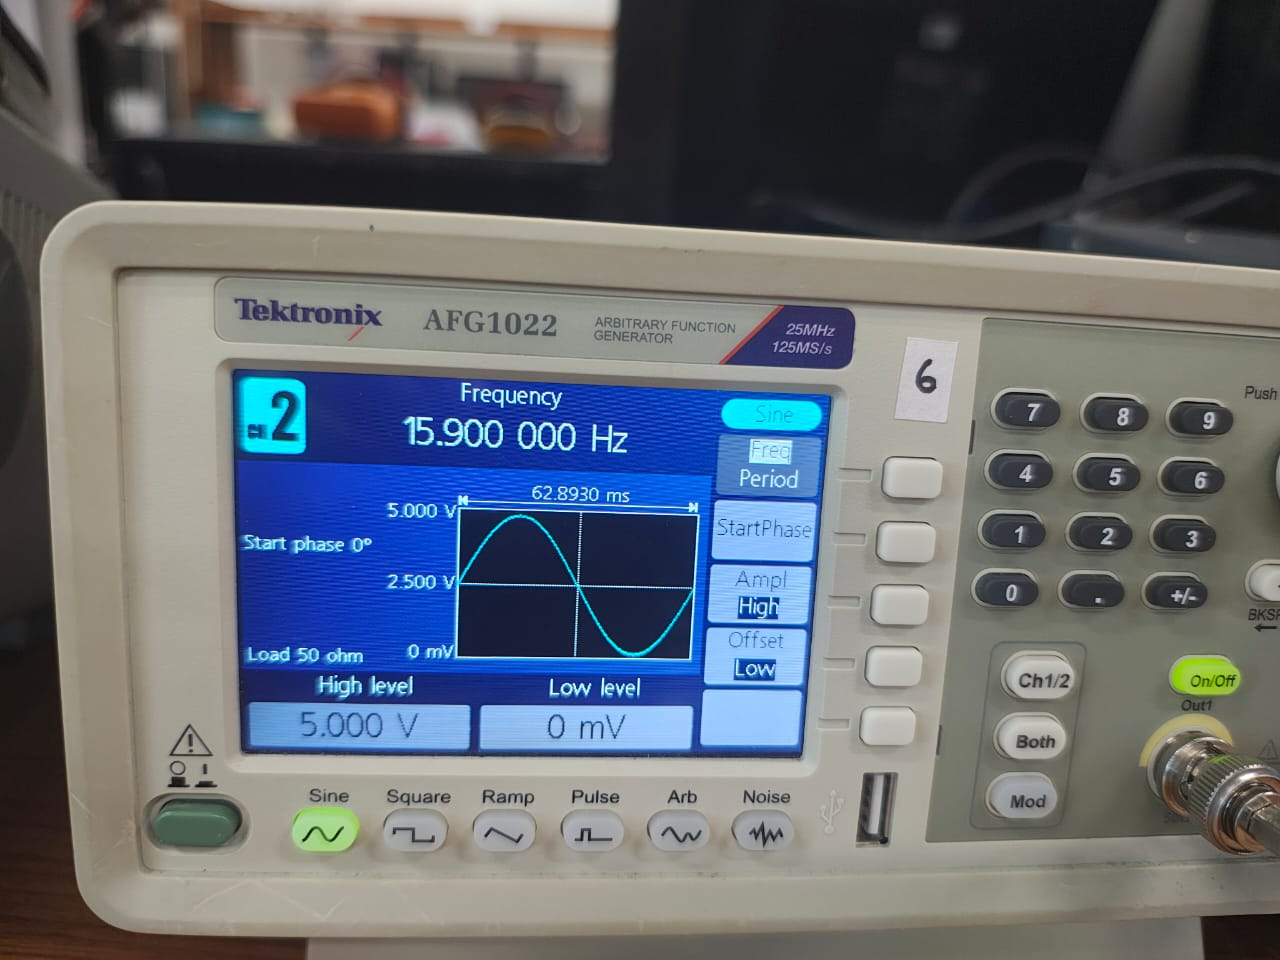
\includegraphics[width=\textwidth]{fig/1w100.jpeg} % Replace with actual file
        \caption{Function Generator Output for w = 100}
    \end{minipage}
\end{figure}

\subsubsection{w = 1000}
\begin{figure}[H]
    \centering
    \begin{minipage}{0.48\textwidth}
        \centering
        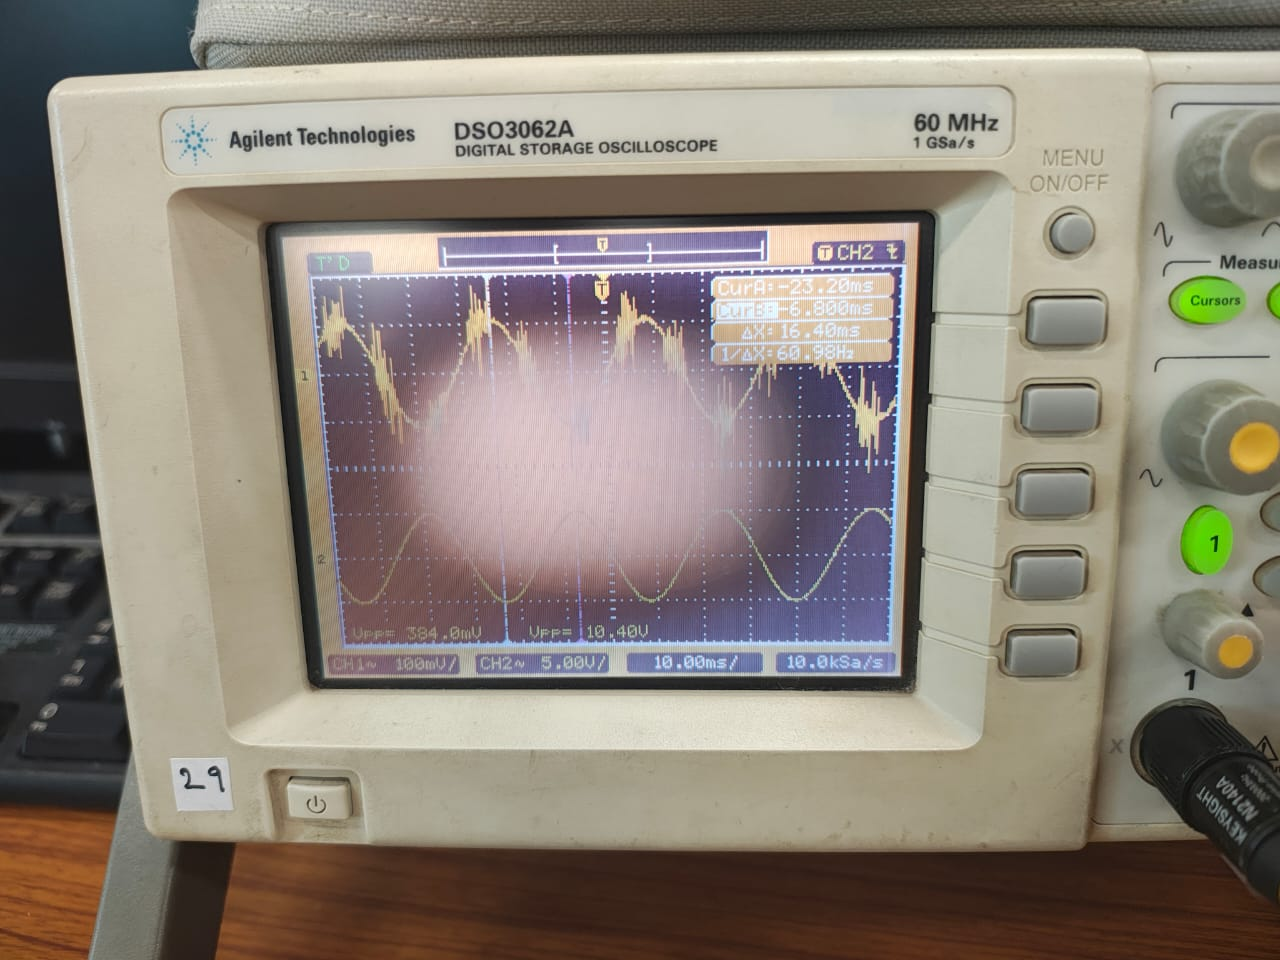
\includegraphics[width=\textwidth]{fig/3w200o.jpeg} % Replace with actual file
        \caption{Oscilloscope Reading for w = 200}
    \end{minipage}
    \hfill
    \begin{minipage}{0.48\textwidth}
        \centering
        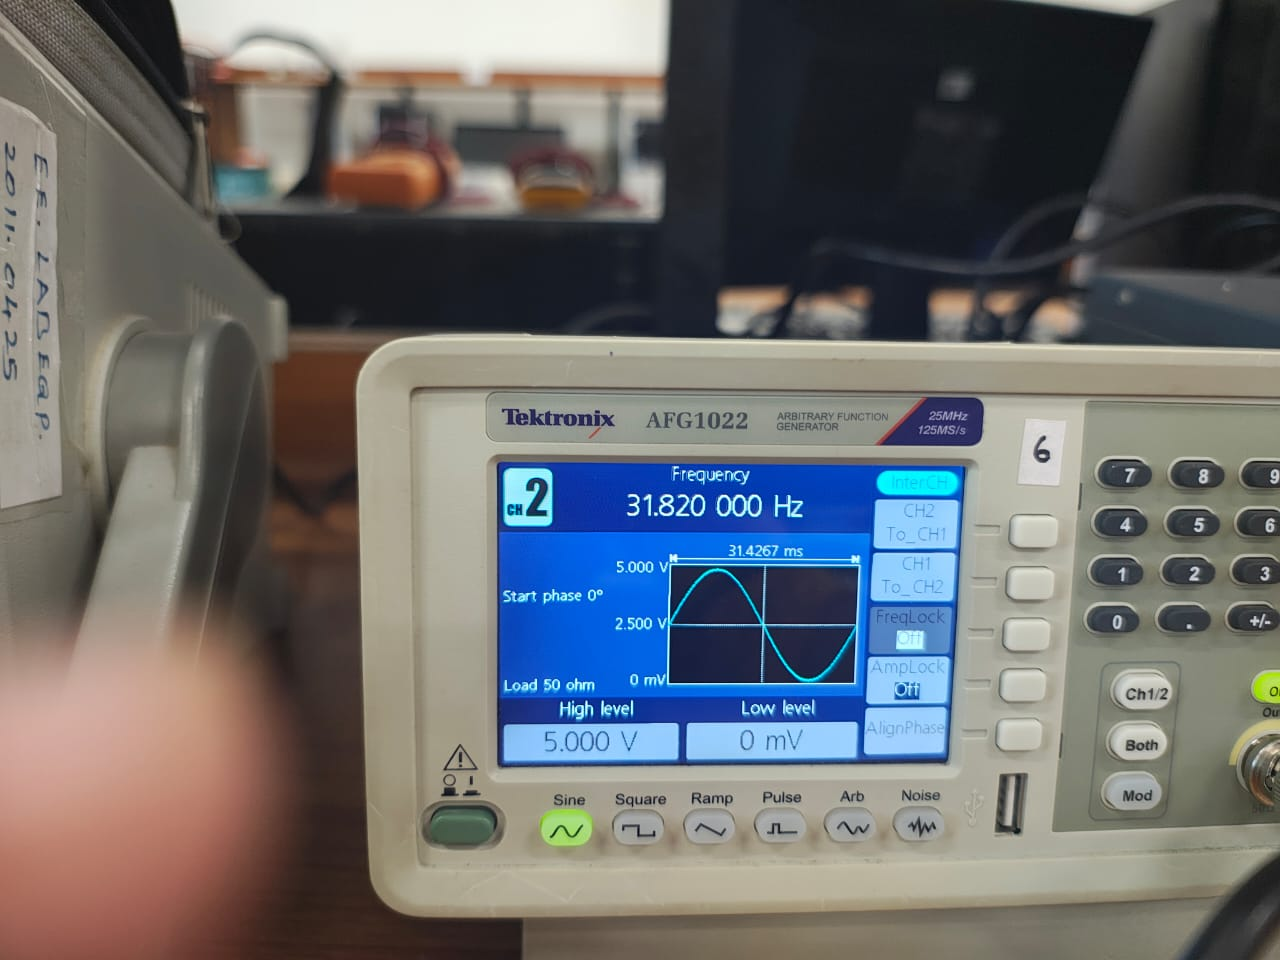
\includegraphics[width=\textwidth]{fig/3w200.jpeg} % Replace with actual file
        \caption{Function Generator Output for w = 200}
    \end{minipage}
\end{figure}
\subsection{Theoretical values}
\begin{align}
\phi &= -17.1^\circ , & \omega &= 10 \text{ rad/s} \\
\phi &= -135^\circ , & \omega &= 100 \text{ rad/s} \\
\phi &= -252.87^\circ , & \omega &= 1000 \text{ rad/s}
\end{align}
\subsection{Magnitude Bode Plot}
\begin{figure}[H]
    \centering
    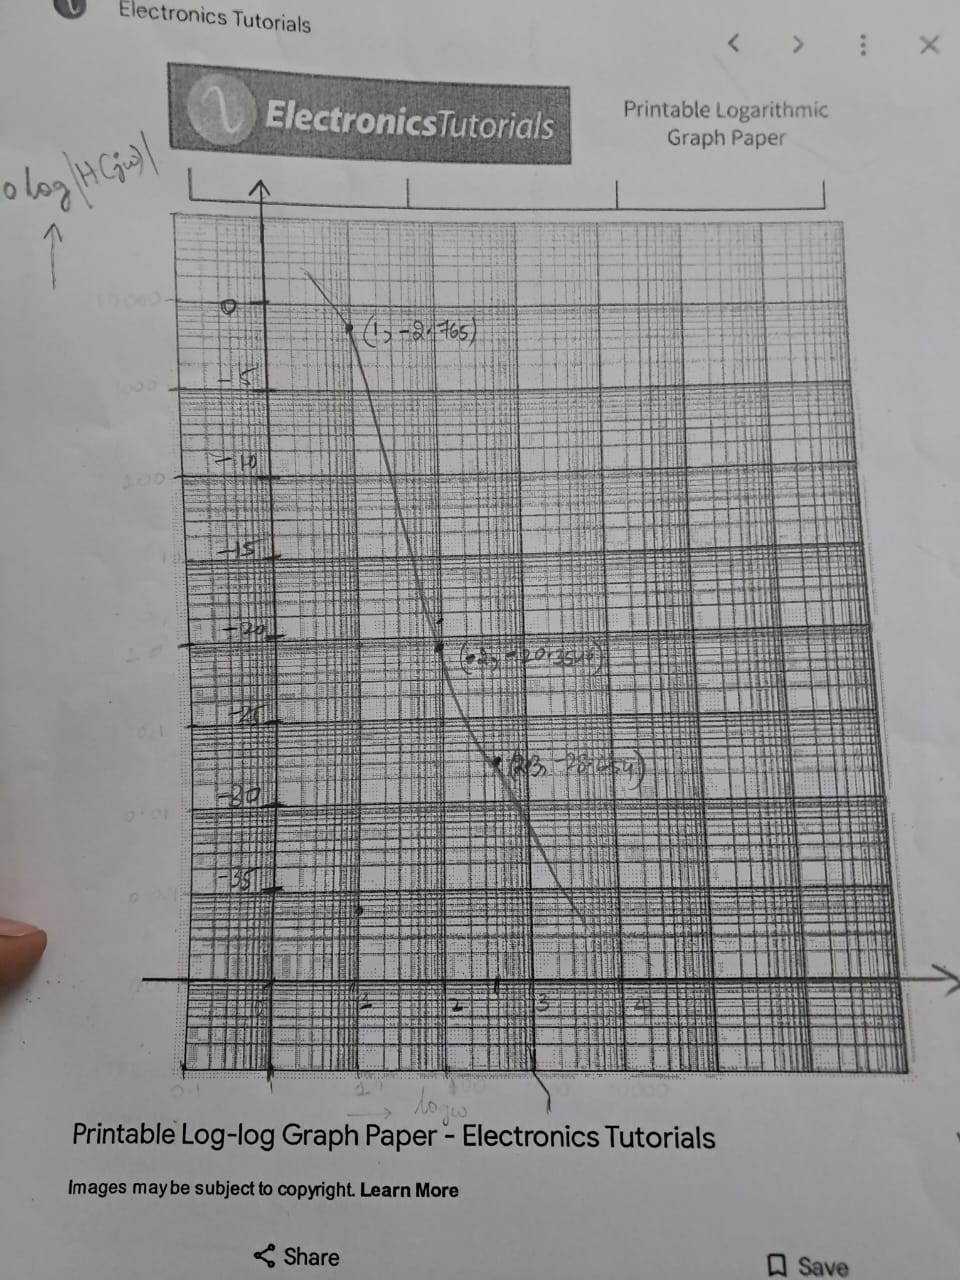
\includegraphics[width=0.7\textwidth]{fig/mbd3.jpeg} % Replace with actual file
    \caption{Magnitude Bode Plot for RC Circuit}
\end{figure}
Magnitude values(measured) are given by:
$$20\log{|H(j\omega)|}=20\log{V_{pp1}/V_{pp2}}$$
\begin{align}
20\log|H(j\omega)| &= -2.765 \text{ dB}, & \omega &= 10 \text{ rad/s} \\
20\log|H(j\omega)| &= -20.3546 \text{ dB}, & \omega &= 100 \text{ rad/s} \\
20\log|H(j\omega)| &= -28.654 \text{ dB}, & \omega &= 1000 \text{ rad/s}
\end{align}
\subsection{Phase Bode Plot}
\begin{figure}[H]
    \centering
    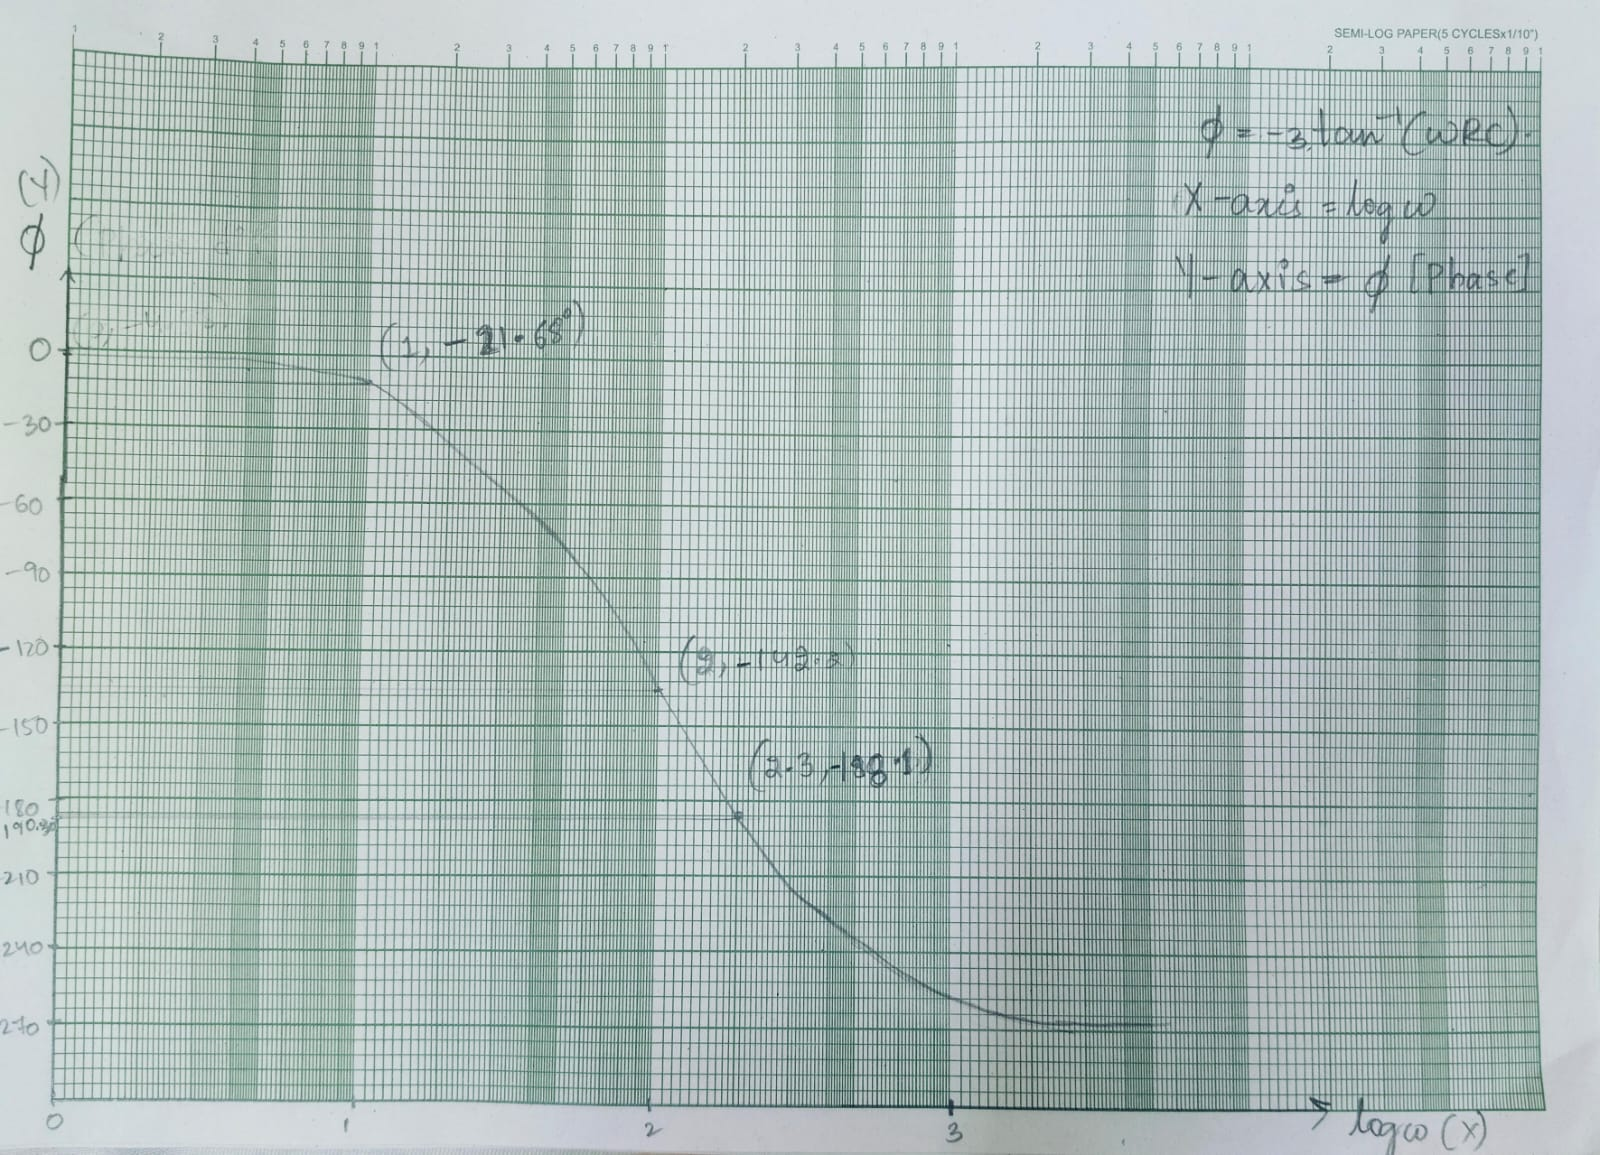
\includegraphics[width=0.7\textwidth]{fig/pbd3.jpeg} % Replace with actual file
    \caption{Phase Bode Plot for RC Circuit}
\end{figure}
Phase difference is given by:
$$\phi = \omega \times \delta t$$
\begin{align}
\phi &= -21.68^\circ, & \omega &= 10 \text{ rad/s} \\
\phi &= -142.2^\circ, & \omega &= 100 \text{ rad/s} \\
\phi &= --188.1^\circ, & \omega &= 200 \text{ rad/s}
\end{align}


\section{Conclusion}
The results demonstrate how cascading RC circuits affects frequency response. The magnitude plot reveals increasing attenuation with cascading, and phase plots show a shift in phase behavior. These findings are essential in filter design and signal processing applications.

\end{document}

